\section{Отпечатъкът на пространство-времето върху поляризираните образи на екзотични компактни обекти}
Тук ще изследваме как природата на пространство-времето около сръхмасивните компактни обекти влияе върху поляризацията на наблюдаваното лъчение. В глава 3 вече представихме досегашните резултати от колаборацията EHT за свръхмасивните обекти M87$^*$ и Sgr A$*$. Бъдещи подобни изследвания (например ngEHT) ще повишат разделителната способност и разширят набора от наблюдавани обекти, но основните затруднения при интерпретацията на резултатите винаги ще останат. А те са именно:\\

\textbf{1)} \emph{Еднозначното определяне на природата на компактният обект, заедно с гравитационната теория, която го описва.}\\

\textbf{2)} \emph{Определянето на физическото състояние на излъчващата среда.}\\

Съвместното решение на горните два въпроса е силно нетривиална задача поради няколко фактора. От една страна, природата на пространство-времето около компактният обект е нелинейно зацепена към магнитохидродинамиката на излъчващата среда, което прави изследването само на един от горните въпроси невъзможно. От друга страна, морфологията на получените образи (въпреки, че съдържа много информация за пространство-времето), както можем да видим от резултатите в глава 7, е силно изродена между драстично различни по природа метрики! Още повече, възможно е съществено различни пространства да притежават математически идентични сенки, което показва че \emph{само} на база морфология \emph{не} може да се фиксира природата на пространство-времето. Следователно са ни нужни допълнителни източници на информация, характеризиращи физиката в непосредствената околност на тези обекти. \\

Един такъв източник е поляризацията на лъчението. Тя характеризира структурата на магнитното поле в излъчващият регион и, още по-важно за нас, разпространението ѝ до наблюдателя се влияе от геометрията на пространство времето (виж уравнението за паралелен пренос (2.14)). Както показа анализът на колаборацията EHT, този допълнителен източник на информация до голяма степен (но не изцяло) снема израждането на задачата за интерпретацията на образите. Мотивирани от това, ние използваме опростеният аналитичен модел, представен в \cite{Narayan2021}, за да изследваме "отпечатъкът"$\,$ на пространство-времето върху поляризацията на получените образи.\\

По-конкретно целим две неща: \\

\textbf{1)} \emph{Да установим дали поляризираните образи на излъчващата среда около екзотични компактни обекти притежават качествено различни свойства, на базата на които можем да ги разграничим от черни дупки на Шварцшилд. Работната ни хипотеза е, че получените поляризирани образи ще са качествено сходни с наблюденията на M87$^*$.}\\

\textbf{2)} \emph{Да дадем количествена оценка за влиянието на пространство-времето върху поляризираните образи.}\\

Ние ще фокусираме нашите разглеждания върху пространствено времевите тунели от глава 5 в стационарният случай, и голи сингулярности на Джанис-Нюман-Уиникър. Сходни изследвания са направени за въртящи се черни дупки на Кер в \cite{Gelles2021}, и за модифицирани теории на гравитацията в \cite{Qin2021}. Някой общи теоретични свойства на поляризираното излъчване около черни дупки на Кер са изследвани в \cite{Himwich2020}, на база класическите работи \cite{Luminet1979}, \cite{Connors1980}, \cite{Chen1991}.\\

Тази глава е структуриране по следният начин: \\

\textbf{1)} В част 7.1 ще представим използваният от нас аналитичният модел на синхотронно излъчващ, намагнитен флуид, движещ се по екваториални орбити и как той може да се използва за построяването на поляризирани образи.\\

\textbf{2)} В части 7.2 и 7.3 ще представим нашите резултати \cite{Delijski2022}, \cite{Deliyski2022} за пространствено-времеви тунели и голи сингулярности. По-конкретно ние изследваме влиянието на геометрията на магнитното поле, инклинацията на наблюдателя, порядъка на полученият образ и параметрите на метриката на пространство-времето.\\

\textbf{3)} В част 7.4 представяме нашите заключения. 

\subsection{Аналитичен модел на синхотронно излъчващ, намагнитен флуид в екваториална орбита}

Нека разгледаме движението на този флуид, около компактен обект, описван от общата статична, сферично симетрична метрика:
\begin{equation}
	ds^2 = - e^{2\nu(r)}dt^2 + e^{2\lambda(r)}dr^2 + R^2(r)\left(d\theta^2 + \sin^2\theta d\phi^2\right).
\end{equation}

Удобно е да изразим поляризацията в собствената отправна система на флуида $\{\hat{e}^\mu_{(a)}\}$, дефинирана с помощта на тетрадата $\{e^\mu_{(a)}\}$ (виж приложение ПРИЛОЖЕНИЕ БАЗИС). За метриката (7.1) тя заема формата:
\begin{equation}
	e_{(t)} = e^{-\nu(r)}\partial_t,\,\, e_{(r)} = e^{-\lambda(r)}\partial_r,\,\, e_{(\theta)} = \frac{1}{R(r)}\partial_{\theta},\,\, e_{(\phi)} = \frac{1}{R(r)\sin\theta}\partial_{\phi}.
\end{equation}

Тогава можем да изразим екваториалната скорост на флуида $\vec{\beta}$, чрез големината $\beta$ и локалната ѝ посока $\chi$:
\begin{equation}
	\vec{\beta} = \beta\left[\cos\chi (r) + \sin\chi (\phi)\right].
\end{equation}
Връзката между тетрадата (7.2) и локалната отправна система на флуида $\{\hat{e}^\mu_{(a)}\}$ се дава с Лоренцовата трансформация $\Lambda^{\,\,\,(b)}_{(a)}$ като:
\begin{equation}
	\hat{e}^\mu_{(a)} = \Lambda^{\,\,\,(b)}_{(a)}e^\mu_{(b)},
\end{equation}
докато всеки вектор $V^{(a)}$ се трансформира с обратната матрица $\Lambda^{\,\,\,(a)}_{(b)}$ според закона:
\begin{equation}
	\hat{V}^{(a)} = \Lambda^{(a)}_{\,\,\,(b)} V^{(b)}.
\end{equation}
Явният израз на матрицата на Лоренц $\Lambda^{(a)}_{\,\,\,(b)}$ се задава с:
\begin{equation}
	\Lambda = \begin{pmatrix}
			\gamma 			 & -\beta\gamma\cos\chi 	    & -\beta\gamma\sin\chi 		   & 0 \\
		-\beta\gamma\cos\chi & (\gamma - 1)\cos^2\chi + 1   & (\gamma - 1)\sin\chi\cos\chi & 0 \\
		-\beta\gamma\sin\chi & (\gamma - 1)\sin\chi\cos\chi & (\gamma - 1)\sin^2\chi + 1   & 0 \\
				0			 &					0			&				0			   & 1
	\end{pmatrix},
\end{equation}
където $\gamma = (1 - \beta^2)^{-1/2}$. Имайки един вектор $\hat{V}^{(a)}$ в локалният базис на флуида, можем да възстановим представянето му в координатния базис $V^\mu$ посредством трансформацията:
\begin{equation}
	V^\mu = \hat{e}^\mu_{(a)}\hat{V}^{(a)}
\end{equation}

В локалният базис на флуида въвеждаме магнитното поле $\vec{B} = (\hat{B}^{(r)},\hat{B}^{(\phi)},\hat{B}^{(\theta)})$ и локалният тримерен импулс на фотоните $\vec{p} = \left(\hat{p}^{(r)},\hat{p}^{(\phi)},\hat{p}^{(\theta)}\right)$. Под действието на магнитното поле, флуида излъчва синхотронно лъчение с вектор на поляризацията $\vec{f}$, задаван в локалният базис на флуида от:
\begin{equation}
	\vec{f} = \frac{\vec{p}\times\vec{B}}{|\vec{p}|},
\end{equation}
където ще се възползваме от калибровъчната свобода за да наложим условието $\hat{f}^{(t)} = 0$. Тогава големината на вектора на поляризацията удовлетворява следното условие:
\begin{equation}
	\hat{f}^{(a)}\hat{f}_{(a)} = \sin^2\zeta|\vec{B}|^2,
\end{equation}
където сме означили със $\zeta$ ъгълът между $\vec{p}$ и магнитното поле $\vec{B}$. Както видяхме в глава 2, в рамките на приближението за геометрична оптика, векторът на поляризацията се пренася паралелно по изотропните геодезични линии на фотоните - т.е. удовлетворява следните уравнения:
\begin{subequations}
	\begin{equation}
		p^\mu\nabla_\mu p^\nu = 0
	\end{equation}
	\begin{equation}
		p^\mu\nabla_\mu f_\mu = 0
	\end{equation}
	\begin{equation}
		p_\mu f^\mu = 0
	\end{equation}
\end{subequations}
В общия случай за да получим поляризацията, измерена от асимптотичен наблюдател, трябва да решим тази система диференциални уравнения за съответните гранични условия. В нашият случай на статични и сферично симетрични метрики обаче, задачата се алгебризира благодарение на наличието на тензор на Килинг-Яно $Y_{\mu\nu}$ от ранк 2. Неговите не-нулеви компоненти се дават от израза:
\begin{equation}
	Y_{\theta\phi} = -Y_{\phi\theta} = R^3(r)\sin\theta
\end{equation} 
В допълнение на $Y_{\mu\nu}$, съществува също и комформен тензор на Килинг-Яно $\tilde{Y}_{\mu\nu}$, представляващ спрягане на $Y_{\mu\nu}$ по Ходж:
\begin{equation}
	\tilde{Y}_{\mu\nu} = \frac{1}{2}\epsilon_{\mu\nu\alpha\beta}Y^{\alpha\beta}.
\end{equation}
Използвайки тези два тензора можем да съставим два интеграла на движението$^1$ $\kappa_1$ и $\kappa_2$, свързани с векторите на импулса $p^\mu$ и поляризацията $f^\mu$ на геодезичната по следният начин:
\begin{subequations}
	\begin{equation}
		\kappa_1 = \frac{1}{2}\tilde{Y}_{\mu\nu}p^\mu f^\nu
	\end{equation}
	\begin{equation}
		\kappa_2 = Y_{\mu\nu}p^\mu f^\nu
	\end{equation}
\end{subequations}
Явните изрази са следните:
\begin{subequations}
	\begin{equation}
		\kappa_1 = R(r)e^{\nu(r) + \lambda(r)}\left( p^tf^r - p^rf^t \right)
	\end{equation}
	\begin{equation}
		\kappa_2 = R^3(r)\sin\theta\left(p^\theta f^\phi - p^\phi f^\theta\right)
	\end{equation}
\end{subequations}
Тези изрази ни позволяват да представим наблюдаваната поляризация, единствено и само чрез граничните условия за геодезичната. Нека разгледаме светлинен лъч, излъчен в точката $x^\mu_s$, с вектор на поляризацията $f^\nu_s$, който достига далечен наблюдател в точката $x^\mu_{\text{obs}}$ с поляризация $f^\mu_{\text{obs}}$. Нека въведем ортонормирана отправна система при наблюдателя, в която да представим измерената от него поляризация. За тази цел ще използваме тетрадата (7.2). Тогава можем да характеризираме проекцията на импулса на лъча чрез два ъгъла $\alpha$ и $\beta$, дефинирани АПЕНДИКС КООРДИНАТИ:
\begin{subequations}
	\begin{equation}
	\sin\alpha = \frac{p^{(\theta)}}{p^{(t)}}
	\end{equation}
	\begin{equation}
		\tan\beta = \frac{p^{(\phi)}}{p^{(r)}},
	\end{equation}
\end{subequations}
които използваме за небесни координати. Понеже те растат обратно-пропорционално на радиалното разстояние, е удобно да ги предефинираме като $x = r\alpha$ и $y = r\beta$. За асимптотичен наблюдател можем да вземем границата $r\rightarrow\infty$ и да получим:
\begin{subequations}
	\begin{equation}
		x = -R(r)p^{(\phi)} = -\frac{p_\phi}{\sin\theta_\text{obs}}
	\end{equation}
	\begin{equation}
		y = R(r)p^{(\theta)} = p_\theta
	\end{equation}
\end{subequations}

Можем сега да изразим константите $\kappa_1$ и $\kappa_2$ чрез проекциите на векторите $f^\mu$ и $p^\mu$ в отправната система на наблюдателя:
\begin{subequations}
	\begin{equation}
		\kappa_1 = R(r)\left(p^{(t)}f^{(r)} - p^{(r)}f^{(t)}\right)
	\end{equation}
	\begin{equation}
		\kappa_2 = R(r)\left(p^{(\theta)}f^{(\phi)} - p^{(\phi)}f^{(\theta)}\right)
	\end{equation}
\end{subequations}
Използвайки съотношението за ортогоналност $p^\mu f_\mu = 0$ можем да решим (7.17) спрямо $f^{(\theta)}$ и $f^{(\phi)}$ и да получим:
\begin{subequations}
	\begin{equation}
		\small
		f^{(\theta)} = \frac{p^{(\theta)}}{(p^{(\theta)})^2 + (p^{(\phi)})^2}\left[-\frac{\kappa_1}{R}\frac{p^{(r)}}{p^{(t)}} + ((p^{(t)})^2 - (p^{(r)})^2)f^{(t)}\right] - \frac{p^{(\phi)}}{(p^{(\theta)})^2 + (p^{(\phi)})^2}\frac{\kappa_2}{R}
	\end{equation}
	\begin{equation}
		\small
		f^{(\phi)} = \frac{p^{(\phi)}}{(p^{(\theta)})^2 + (p^{(\phi)})^2}\left[-\frac{\kappa_1}{R}\frac{p^{(r)}}{p^{(t)}} + ((p^{(t)})^2 - (p^{(r)})^2)f^{(t)}\right] + \frac{p^{(\theta)}}{(p^{(\theta)})^2 + (p^{(\phi)})^2}\frac{\kappa_2}{R}
	\end{equation}
\end{subequations}

Тези изрази могат да се опростят за асимототичен наблюдател, възползвайки се от още един интеграл на движението, генериран от тензора на Килинг-Яно. Неговият квадрат представлява тензора на Килинг $K_{\mu\nu} = Y_{\mu\alpha}Y_{\nu}^{\,\,\,\alpha}$, който генерира запазващата се величина $C = K_{\mu\nu}p^\mu p^\nu$. Явната му форма е:
\begin{equation}
	C =  R^4(r)\left[\left(p^{\theta}\right)^2 + \sin^2\theta \left(p^{\phi}\right)^2\right] = R^2(r)\left[\left(p^{(\theta)}\right)^2 + \left(p^{(\phi)}\right)^2\right].
\end{equation}
Използвайки този интеграл на движението и условието за изотропност на светлинните геодезични $p_\mu p^\mu = 0$ можем да видим, че в границата $r\rightarrow\infty$, членовете в (7.17), пропорционални на $f^{(t)}$ изчезват. Тогава използвайки дефиницията на небесните координати $x$ и $y$ (7.16), получаваме изразите за компонентите на вектора на поляризацията, измерени от асимптотичен наблюдател:
\begin{subequations}
	\begin{equation}
		f^x = \frac{x\kappa_1 + y\kappa_2}{x^2 + y^2}
	\end{equation}
	\begin{equation}
		f^y = \frac{y \kappa_1 - x\kappa_2}{x^2 + y^2}.
	\end{equation}
\end{subequations}
Можем допълнително да нормираме тези изрази така, че измереният вектор на поляризацията да има големина единица:
\begin{subequations}
	\begin{equation}
		f^x_\text{obs} = \frac{x\kappa_1 + y\kappa_2}{\sqrt{(x^2 + y^2)(\kappa_1^2 + \kappa_2^2)}}
	\end{equation}
	\begin{equation}
		f^y_\text{obs} = \frac{y \kappa_1 - x\kappa_2}{\sqrt{(x^2 + y^2)(\kappa_1^2 + \kappa_2^2)}}.
	\end{equation}
\end{subequations}

По този начин получаваме изрази за наблюдаваната поляризация на безкрайност, зависещи единствено от интегралите на движение $\kappa_1$ и $\kappa_2$, и проекцията на фотонната траектория върху екрана на наблюдателя $(x,y)$. Самите $\kappa_1$ и $\kappa_2$ могат да се определят само от началните данни за поляризацията - т.е. от параметрите на физичния процес, пораждащ лъчението. Трансформирайки вектора на поляризацията от собствената отправна система на флуида, към тетрадата (7.2) и замествайки в (7.17) получаваме изрази за $\kappa_1$ и $\kappa_2$, които зависят само от началните данни в собствената отправна система на флуида:
\begin{subequations}
	\begin{equation}
		\kappa_1 = \gamma R(r_s)\left[\hat{p}^{(t)}\hat{f}^{(r)} + \beta\left(\hat{p}^{(r)}\hat{f}^{(\theta)} - \hat{f}^{(r)}\hat{p}^{(\theta)}\right)\right]
	\end{equation}
	\begin{equation}
		\kappa_2 = \gamma R(r_s)\left[\left(\hat{p}^{(\theta)}\hat{f}^{(\phi)} - \hat{f}^{(\theta)}\hat{p}^{(\phi)}\right) - \beta \hat{p}^{(t)} \hat{f}^{(\phi)}\right]
	\end{equation}
\end{subequations}

За да изследваме структурата на поляризацията, ние използваме две наблюдаеми величини - интензитета и посоката на вектора на поляризацията. Интензитета е пропорционален на големината на вектора на поляризацията, но трябва също да отчетем и допълнителни ефекти, свързани с феноменологията на синхотронното излъчване. Този интензитет зависи от ъгълът между магнитното поле и импулса на фотона в отправната система на флуида като $I\propto(\sin\zeta)^{1 + \alpha_\nu}$. Понеже има излъчване от всяка точка на диска (т.е. то е на единица обем), интензитетът трябва също да се коригира с дължината на геодезичната през зоната на излъчване $\ell_p$. За оптически и геометрично тънък диск, тази дължина може да се изрази като:
\begin{equation}
	\ell_p = \bigg\vert\frac{\hat{p}^{(t)}}{\hat{p}^{(\theta)}}\bigg\vert H,
\end{equation}
където $H$ е дебелината на диска. Освен това, излъчването силно се влияе от релативисткият ефект на Доплер. Това се отчита с допълнителният множител $g^{3 + \alpha_\nu}$, дефиниран посредством червеното отместване:
\begin{equation}
	g = \frac{E_\text{obs}}{E_s} = \frac{1}{\hat{p}^{(t)}}.
\end{equation}
Така, приемайки нормализацията (7.21), можем да запишем интензитетът $I$ на поляризацията, измерена от наблюдател на безкрайност като:
\begin{equation}
	I = g^{3 + \alpha_\nu}\ell_p(\sin\zeta)^{1 + \alpha_\nu},
\end{equation}
с точност до константа. Моделите на M87$^*$ подкрепят стойността $\alpha_\nu = 1$, която ще използваме в нашите изследвания тук. Можем също да дефинираме компонентите на електричното поле $\{E^x, E^y\}$ като:
\begin{subequations}
	\begin{equation}
		E^x_{\text{obs}} = g^2\sqrt{\ell_p}\sin\zeta f^x_\text{obs},
	\end{equation}
	\begin{equation}
		E^y_\text{obs} = g^2\sqrt{\ell_p}\sin\zeta f^x_\text{obs},
	\end{equation}
	\begin{equation}
		I = (E^x_\text{obs})^2 + (E^y_\text{obs})^2.
	\end{equation}
\end{subequations}
Последно, посоката на поляризацията ще дефинираме посредством \emph{ъгълът на завъртане на електричният вектор} $EVPA$, дефиниран като:
\begin{equation}
	EVPA = \arctan\left(-\frac{f^x_\text{obs}}{f^y_\text{obs}}\right)
\end{equation}

\subsection{Поляризация от статични и стационарни пространствено - времеви тунели}
В тази част ще приложим описаният до тук можел на излъчващ намагнитен флуид за да получим наблюдаваните поляризирани образи на орбити около пространствено-времеви тунели в стационарният случай. Те зависят от набор физични параметри, които могат да бъдат разделени на два типа:\\

\textbf{1)} Такива, определящи състоянието на излъчващата среда. В нашият опростен модел те включват геометрията на магнитното поле, и скоростта на флуида.\\

\textbf{2)} Такива, свързани със свойствата на пространство-времето. Това са параметрите на самата метрика, иклинацията на наблюдателя и радиуса на излъчващата орбита.\\

С оглед работната ни хипотеза, че получените тук поляризирани образи ще са качествено сходни с наблюдаваните за M87$^*$, ще се фокусираме най-вече върху параметрите на задачата, за които отклоненията на тези образи от наблюдаваните е най-малко. Следователно ще се наблегнем върху ниски инклинации $i = 20^\circ$ и орбити, намиращи се в зоната на силна гравитация. Предполагаме, че флуидът се движи по тези орбити, видимо по посока на часовниковата стрелка, както при M87$^*$ \cite{EHT_M87_V}, и се ограничаваме до тези, близки до ISCO за Шварцшилд, и орбитата $r_s = 4.5M$ (съответстваща на видимия радиус на излъчващият пръстен, наблюдаван при М87$^*$). \\

За да фиксиране на геометрията на магнитното поле, ще се възползваме от резултатите на предишни изследвания \cite{Narayan2021}. Те демонстрираха, моделирайки централният обект като черна дупка на Шварцшилд, че чисто вертикални, радиални или азимутални полета \emph{не} са подходящи за възпроизвеждане на наблюдаваните от EHT поляризирани образи на M87$^*$. Видимата асиметрия в образа се дължи на комбинация от релативискти ефект на Доплер и аберация, както и от ефекта на лещата. За вертикални магнитни поле тези ефекти се конкурират.\\

За флуид, въртящ се видимо по часовниковата стрелка (както \cite{EHT_M87_V} заключи) или радиално навътре (както е естествено за акреционни процеси), аберацията надделява, водейки до нарастване на интензитета в съответно в лявата или долната част на образа. Това е в противоречие с наблюденията на М87$^*$, където максимума в интензитета е от дясната страна на образа. Подобен ефект се забелязва при неподвижен флуид, благодарение на ефекта на лещата - интензитетът има максимум в долната част на образа. Това показва, че магнитното поле в излъчващата среда около M87$^*$ трябва да има значителна екваториална компонента. \\

Разглеждайки такива полета, \cite{Narayan2021} показват, че ефекта на Доплер и аберацията си подпомагат, което възпроизвежда максимума на интензитета в дясната страна на образа. Също показаха, че изцяло радиално или азимутално поле не може да възпроизведе характерното за M87$^*$ завъртане на поляризационният вектор. Те дават оценката, че смесено екваториално магнитно поле от вида $B = (\hat{B}^{(r)},\hat{B}^{(\phi)},\hat{B}^{(\theta)}) = (0.87,0.5,0)$ най-добре описва наблюденията на M87$^*$. Тази оценка също и определя посоката на скоростта на флуида. В най-вътрешните зони на акреционният диск и най-вероятно магнитното поле и вектора на скоростта на флуида да са паралелни или анти-паралелни. В нашият случай тези две възможности пораждат една и съща поляризация, поради което ще изберем само анти-паралелната конфигурация.\\

Ние ще се спрем на кратко върху вертикалните полета, за да покажем, че описаното в \cite{Narayan2021} поведение се запазва и при пространствено-времевите тунели, след което ще разглеждаме само екваториални полета. За целта ни е нужен начин за пресмятане на импулсите на фотони, съответстващи на образа на излъчващият флуид, когато те попаднат върху него. В \cite{Narayan2021} са използвали аналитично приближение за решението на уравнение (6.5). Вместо това ние ще използваме численият код Mjølnir (виж приложение КОД), за пресмятането на тези импулси. По-конкретно: за даден образ на излъчваща орбита с радиус $r_s$, използваме процедурата от глава 6 за извличане на прицелните параметри от $\{\xi,\eta\}$ от координатите на образа $\{x, y\}$ (виж приложение КООРДИНАТИ БАЗИС). След което подаваме тези прицелни параметри като начално условие на Mjølnir, и пропагираме фотоните докато не достигнат $r = r_s$, при което извличаме техните импулси в координатен базис $p_\mu$. Разлагаме ги в локалната тетрада (7.2) при $r = r_s$, след което прилагаме Лоренцовата трансформация (7.5) и пресмятаме поляризацията чрез (7.8), за фиксирано магнитно поле $\vec{B}$. Имайки $\vec{f}$ в отправната система на флуида, можем да пренесем тази поляризация до наблюдателя на безкрайност, използвайки константите $\kappa_1$ и $\kappa_2$, и да пресметнем наблюдаемите величини - интензитетът $I$ и наклона на поляризационния вектор $EVPA$.
\subsubsection{Поляризация на директните образи}
Като начален етап от изследванията ни, разглеждаме случая за вертикално магнитно поле. Целим да установим дали такова поле в пространство-време на тунел, също води до поляризирани образи, които са качествено различни от наблюдаваните за M87$^*$. Ефекта на аберацията, отговорен за появата на максимума на излъчване от лявата страна на образа е чисто кинематичен, и ще присъства независимо от природата на пространство-времето. Важено е обаче, да проверим дали ефекта на лещата в околността на тунела няма да предизвика обратният ефект, и да измести видимия максимум на интензитета, спрямо черни дупки на Шварцшилд. Разглеждаме орбитите $r_s = 6M$ и $r_s = 4.5M$. Варираме параметъра $\gamma\in[0,3]$ и на фигура \ref{WH_pol_vert_field} сравняваме получената поляризация на съответните образи.\\

Виждаме, че тя силно наподобява тази при черни дупки на Шварцшилд с разликата, че интензитетът на поляризацията е по-малък, и намалява с увеличаване на параметъра $\gamma$ и видимата позиция на образите е леко изместена. Важното е, че разпределението на този интензитет и наклона следват тези при Шварцшилд. Следователно можем да заключим, че и в пространство-времето на тунел, вертикалните магнити полета пораждат образи, които не са съвместими с наблюденията на М87$^*$. Поради тази причина ще фокусираме разглежданията си от тук нататък само върху екваториални магнитни полета. \newpage

\begin{figure}[!htb]
	\begin{subfigure}{7cm}
		\hspace{0.0em}
		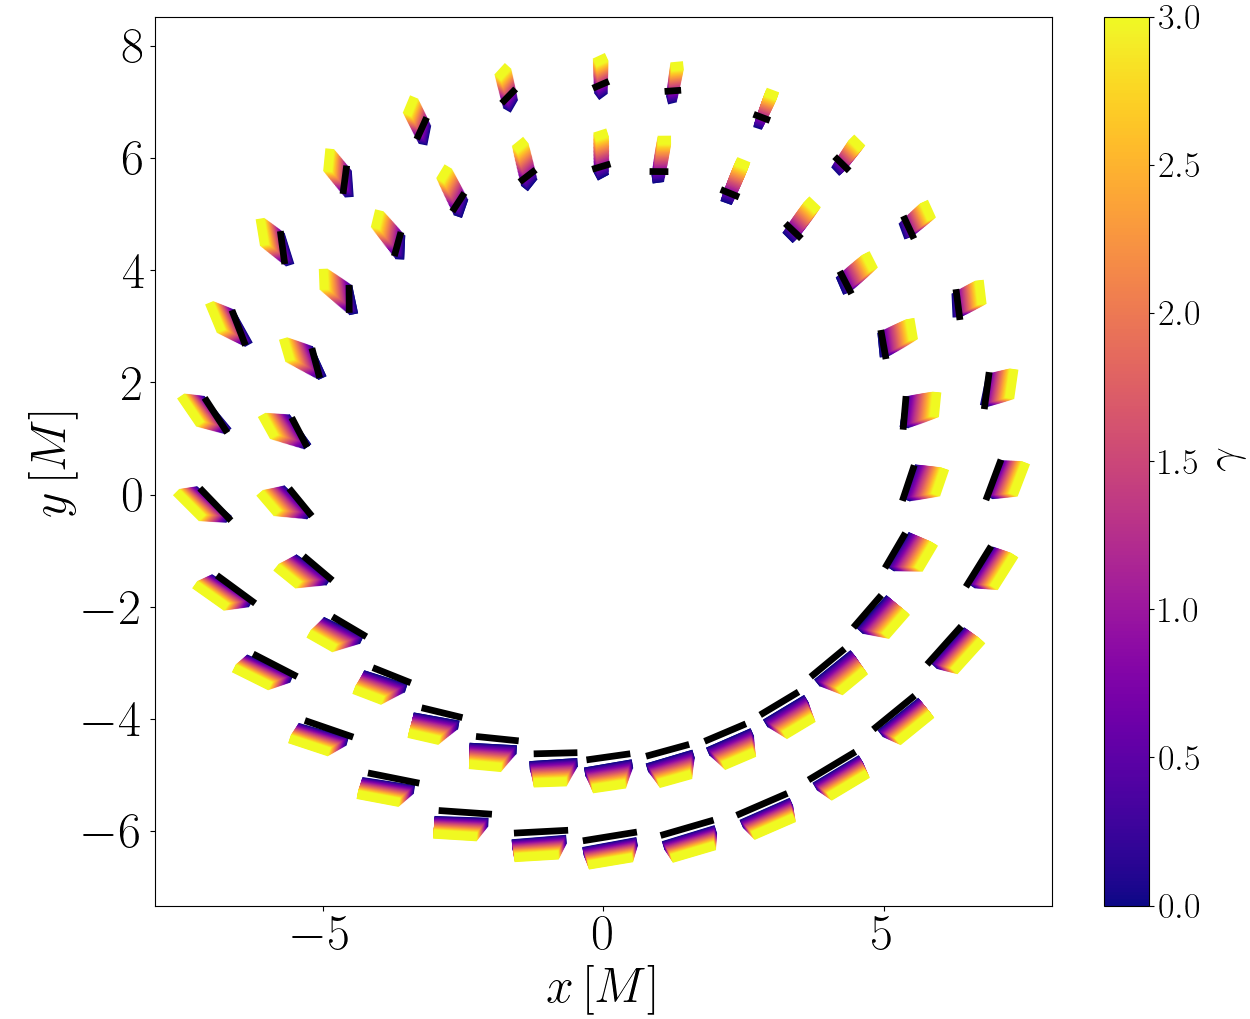
\includegraphics[scale = 0.23]{WH_alpha_Vert_Field.png}
		\caption{$\vec{B} = [0, 1, 0]$, $\beta = 0.3$, $\chi = -150^\circ$.} 
	\end{subfigure}\,\,\,
	\begin{subfigure}{7cm}
		\hspace{0.2em}
		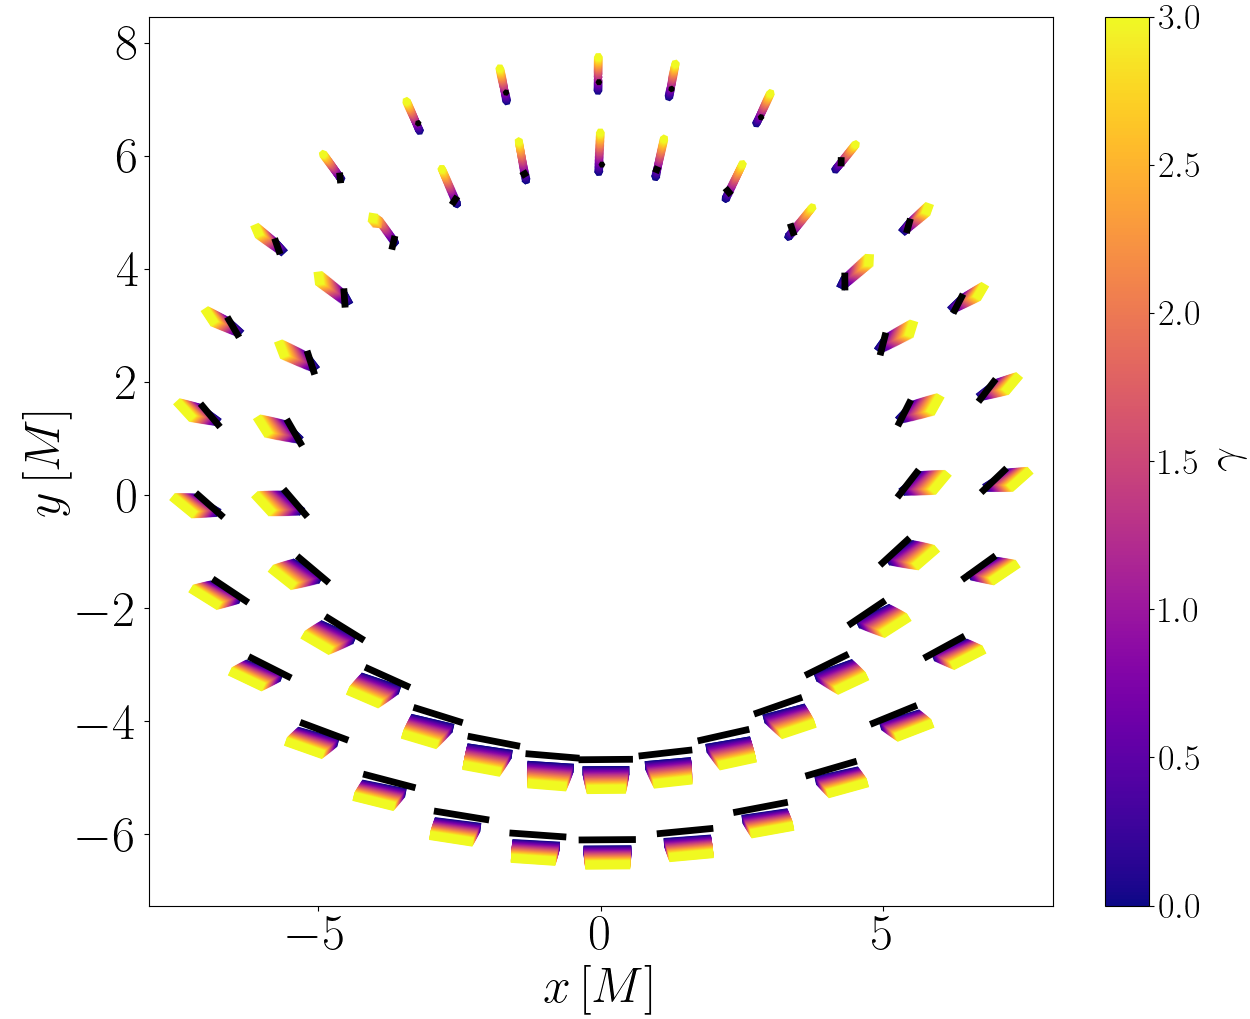
\includegraphics[scale = 0.23]{WH_alpha_Vert_Field_beta_zero.png}
		\caption{$\vec{B} = [0, 1, 0]$, $\beta = 0$, $\chi = -150^\circ$.}
	\end{subfigure}
	\caption[Поляризирани образи около пространствено - времеви тунели за вертикално магнитно поле.]{\small Построените поляризирани образи на орбитите $r_s = 6M$, $r_s = 4.5M$ около пространствено - времеви тунели за вертикално магнитно поле и $\gamma \in[0,3]$ и $i = 20^\circ$. Черните линии съответстват на черна дупка на Шварцшилд.} 
	\label{WH_pol_vert_field}
\end{figure}

На фигура \ref{WH_pol_eq_field} сме начертали поляризираните образи на същите две орбити за 3 репрезантативни конфигурации на екваториално магнитно поле, варирайки параметъра на метриката $\gamma \in[0,3]$. Отново наблюдаваме качествено сходен характер с черни дупки на Шварцшилд. Максимумът на интензитета се концентрира в дясната страна на образа и наклона следва същата зависимост с малки отклонения за всички стойности на $\gamma$. \\

\emph{Следователно можем да заключим, че директните образи се влияят слабо от природата на пространство-времето, разглеждайки ниски инклинации.}

\begin{figure}[!htb]
	\centering
	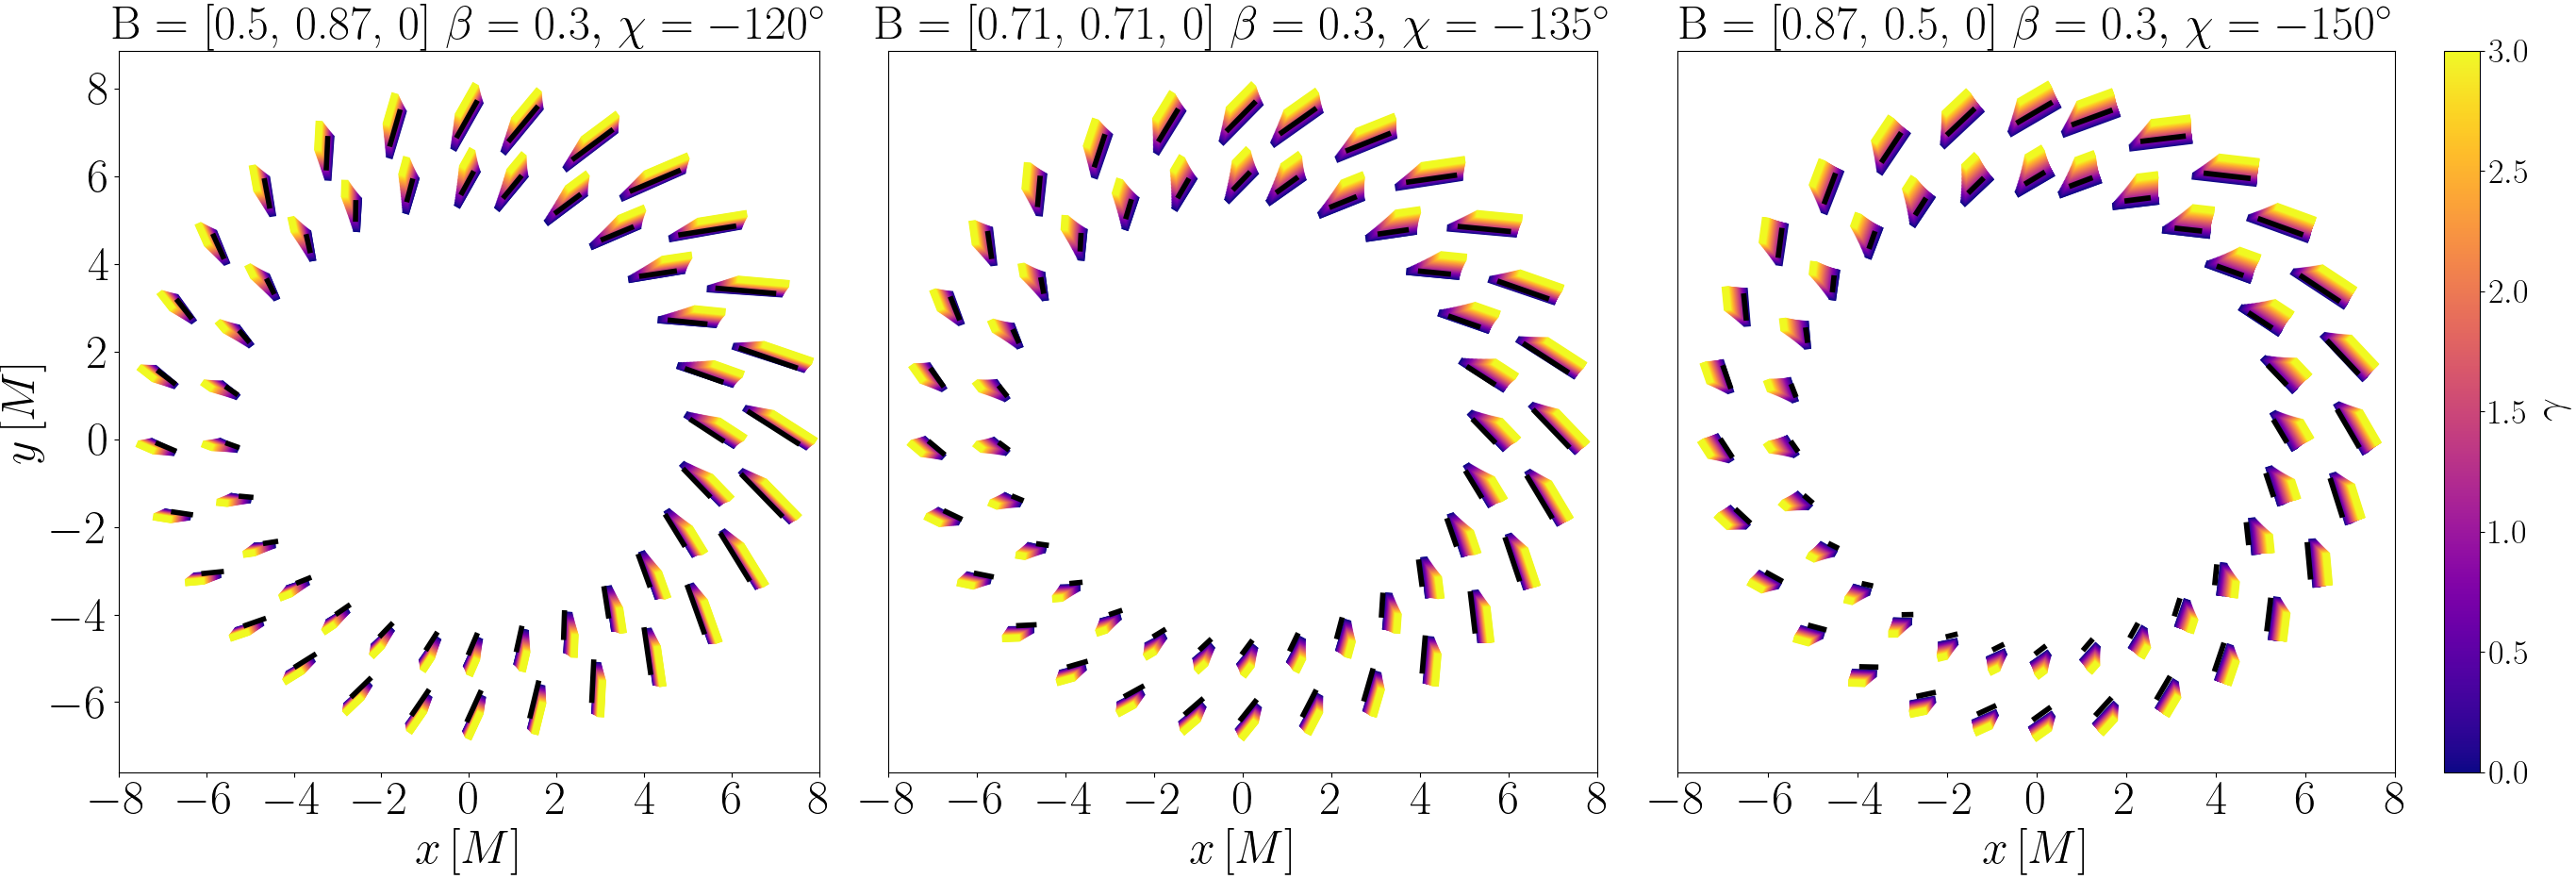
\includegraphics[scale = 0.2]{WH_alpha_Eq_Field.png}
	\caption[Поляризирани директни образи около пространствено - времеви тунели за екваториално магнитно поле.]{\small Построените директни поляризирани образи на орбитите $r_s = 6M$, $r_s = 4.5M$ около пространствено - времеви тунели за екваториално магнитно поле и $\gamma \in[0,3]$ и $i = 20^\circ$. Черните линии съответстват на черна дупка на Шварцшилд.} 
	\label{WH_pol_eq_field}
\end{figure}

\newpage

Имайки предвид този резултат, нека сега изследваме \emph{количествената} разлика в поляризацията. Понеже целим дали можем да различим тези две пространства чрез наблюдения, ще сравняваме поляризацията при една и съща видима точка върху равнината на наблюдение $\{x,y\}$, вместо при еднакви радиуси на излъчване $r_s$. Поради различната степен на фокусировка в различните пространства, радиуса на излъчване $r_s$ в този случай ще варира по образа. Обаче ако се ограничим само до директните, това вариране е минимално.\\

На фигура \ref{WH_delta_r6} е показан анализа ни на поляризираните образи, разположени при координати $\{x,y\}$, съответстващи на орбитата $r_s = 6M$ за пространство-време на Шварцшилд (ще бележим тези образи в текста с обозначението $\{x,y\}\vert_{6M, \text{Schw}}$). За всеки образ чертаем интензитета $I$, и наклона $EVPA$ на поляризационният вектор, като функция на азимуталната координата $\delta = \arctan(y / x)$. Освен това чертаем и отклоненията от Шварцшилд $\Delta I = I_{\text{WH}} - I_{\text{Schw}}$ и $\Delta EVPA = EVPA_\text{WH} - EVPA_\text{Schw}$ за всяка точка от образа.

\begin{figure}[!htb]
	\centering
	\begin{subfigure}{12cm}
		\hspace{-2cm}
		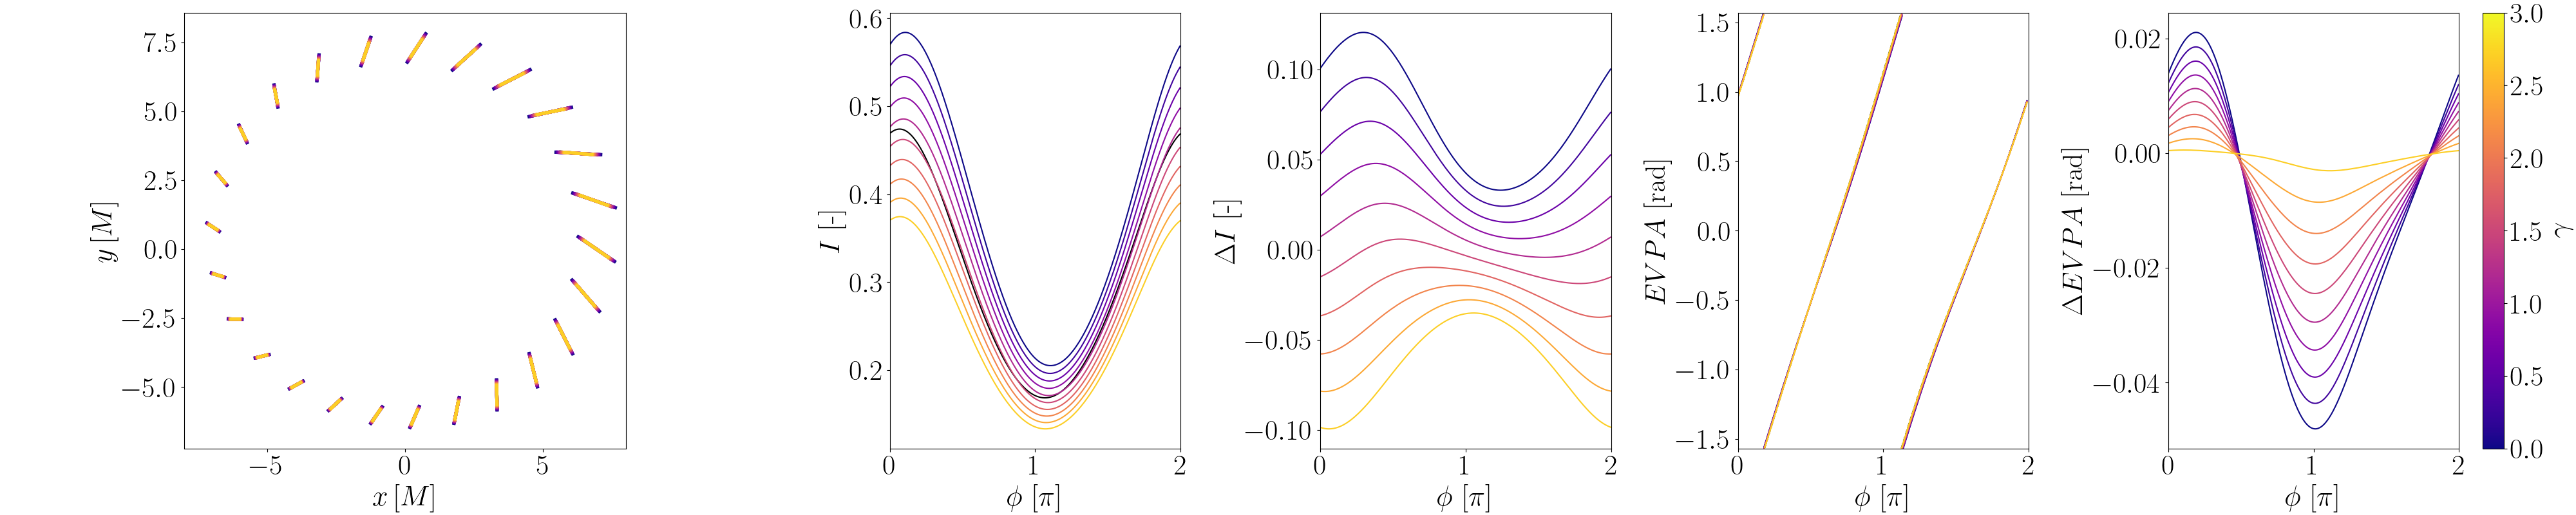
\includegraphics[scale = 0.15]{WH_delta_fig_B_0.5_0.87_0_20_deg_r6.png}
		\caption{$\vec{B} = [0.5, 0, 0.87]$, $\beta = 0.3$, $\chi = -120^\circ$.} 
	\end{subfigure}\\
	\begin{subfigure}{12cm}
		\hspace{-2cm}
		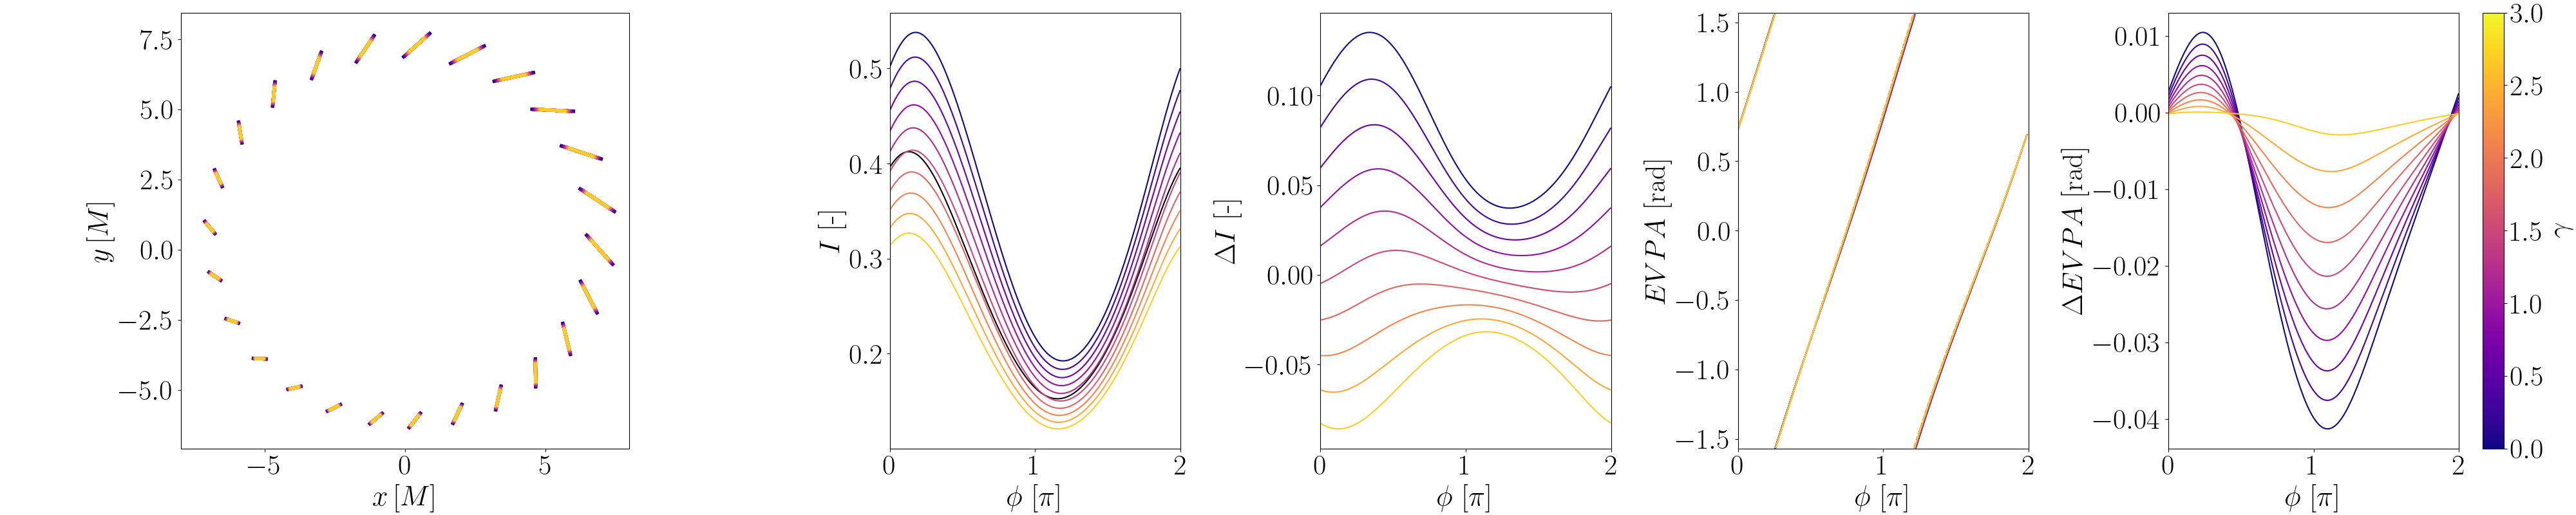
\includegraphics[scale = 0.15]{WH_delta_fig_B_0.71_0.71_0_20_deg_r6.png}
		\caption{$\vec{B} = [0.71, 0, 0.71]$, $\beta = 0.3$, $\chi = -135^\circ$.}
	\end{subfigure}\\
	\begin{subfigure}{12cm}
		\hspace{-2cm}
		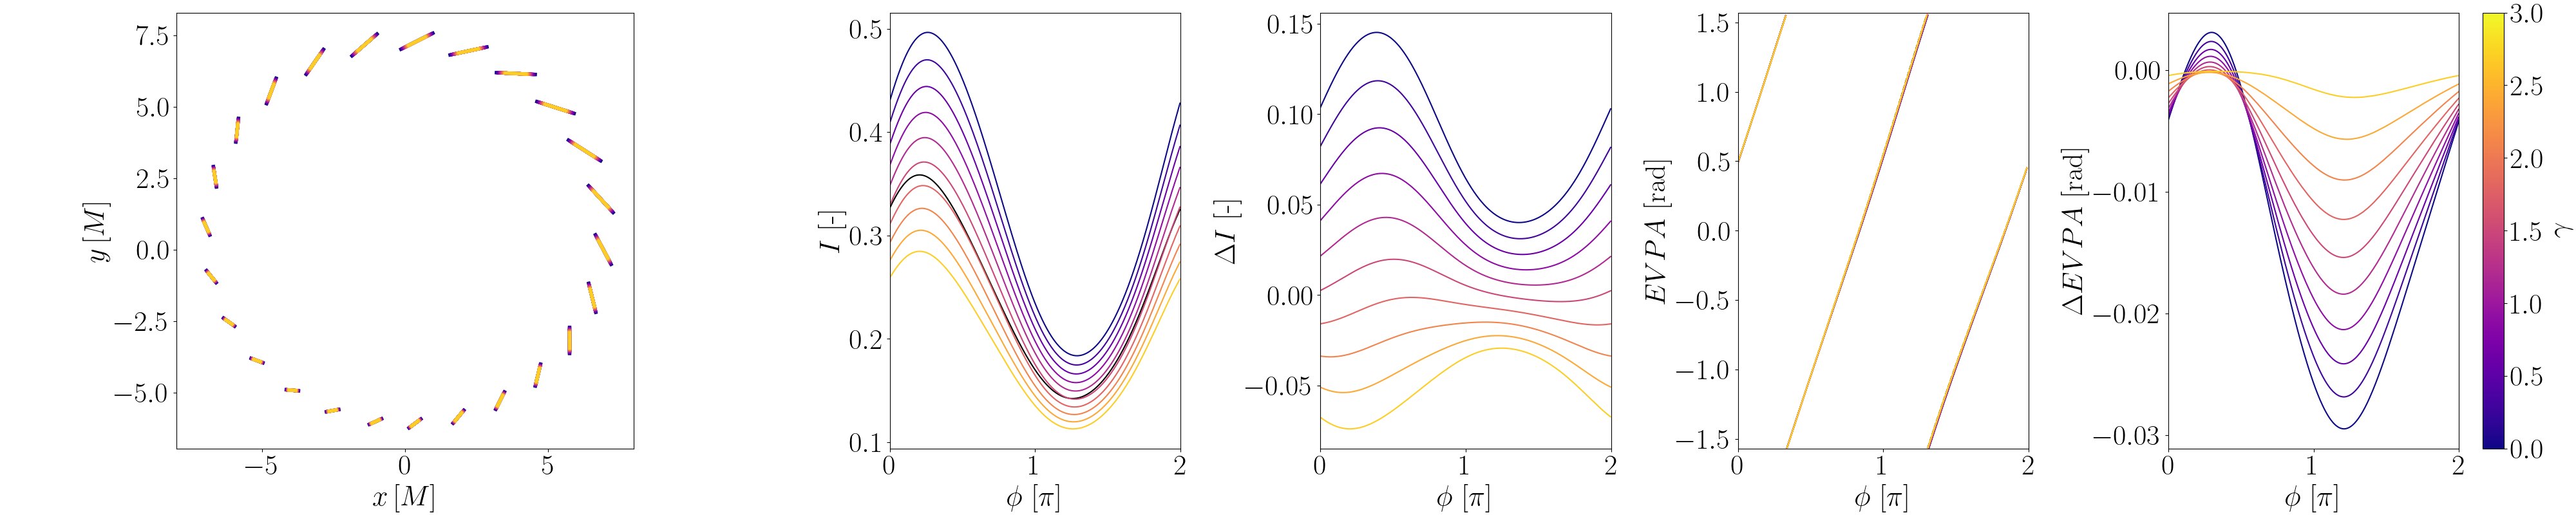
\includegraphics[scale = 0.15]{WH_delta_fig_B_0.87_0.5_0_20_deg_r6.png}
		\caption{$\vec{B} = [0.87, 0, 0.5]$, $\beta = 0.3$, $\chi = -150^\circ$.}
	\end{subfigure}
	\caption[Профили на отклоненията на поляризираните образи oт тип $\{x,y\}\vert_{6M, \text{Schw}}$, за $i = 20\deg$.]{\small Профили на отклоненията на поляризираните образи от тип $\{x,y\}\vert_{6M, \text{Schw}}$, за $i = 20\deg$. Черната крива на $I(\phi)$ съответства на черни дупки на Шварцшилд.} 
	\label{WH_delta_r6}
\end{figure}

\newpage

Виждаме, че за всяко $\gamma$, профилът на интензитета и наклона на поляризационният вектор имат качествено същото поведение като при Шварцшилд, и големината на отклоненията им не е значителна. Освен това забелязваме, че за малки $\gamma$, $\Delta I$ положително, докато за големи $\gamma$ - отрицателно. Това подсказва, че съществува критична стойност $\gamma_\text{crit}^{(1)}$, при която отклоненията в интензитета на поляризацията са най-малки. Обратното поведение наблюдаваме при $\Delta EVPA$. Тогава можем да заключим, че съществува втора критична стойност $\gamma_\text{crit}^{(2)}$, при която отклоненията в наклона на поляризационният вектор са минимални. На фигура \ref{WH_max_deviation_20_deg} изследваме тези критични стойности по-подробно. За всяка стойност на $\gamma$ пресмятаме максималните по амплитуда $\Delta I$ и $\Delta EVPA$, след което ги чертаем като функция на $\gamma$, за да оценим $\{\gamma_\text{crit}^{(1)}, \gamma_\text{crit}^{(2)}\}$.

\begin{figure}[!htb]
		\centering
		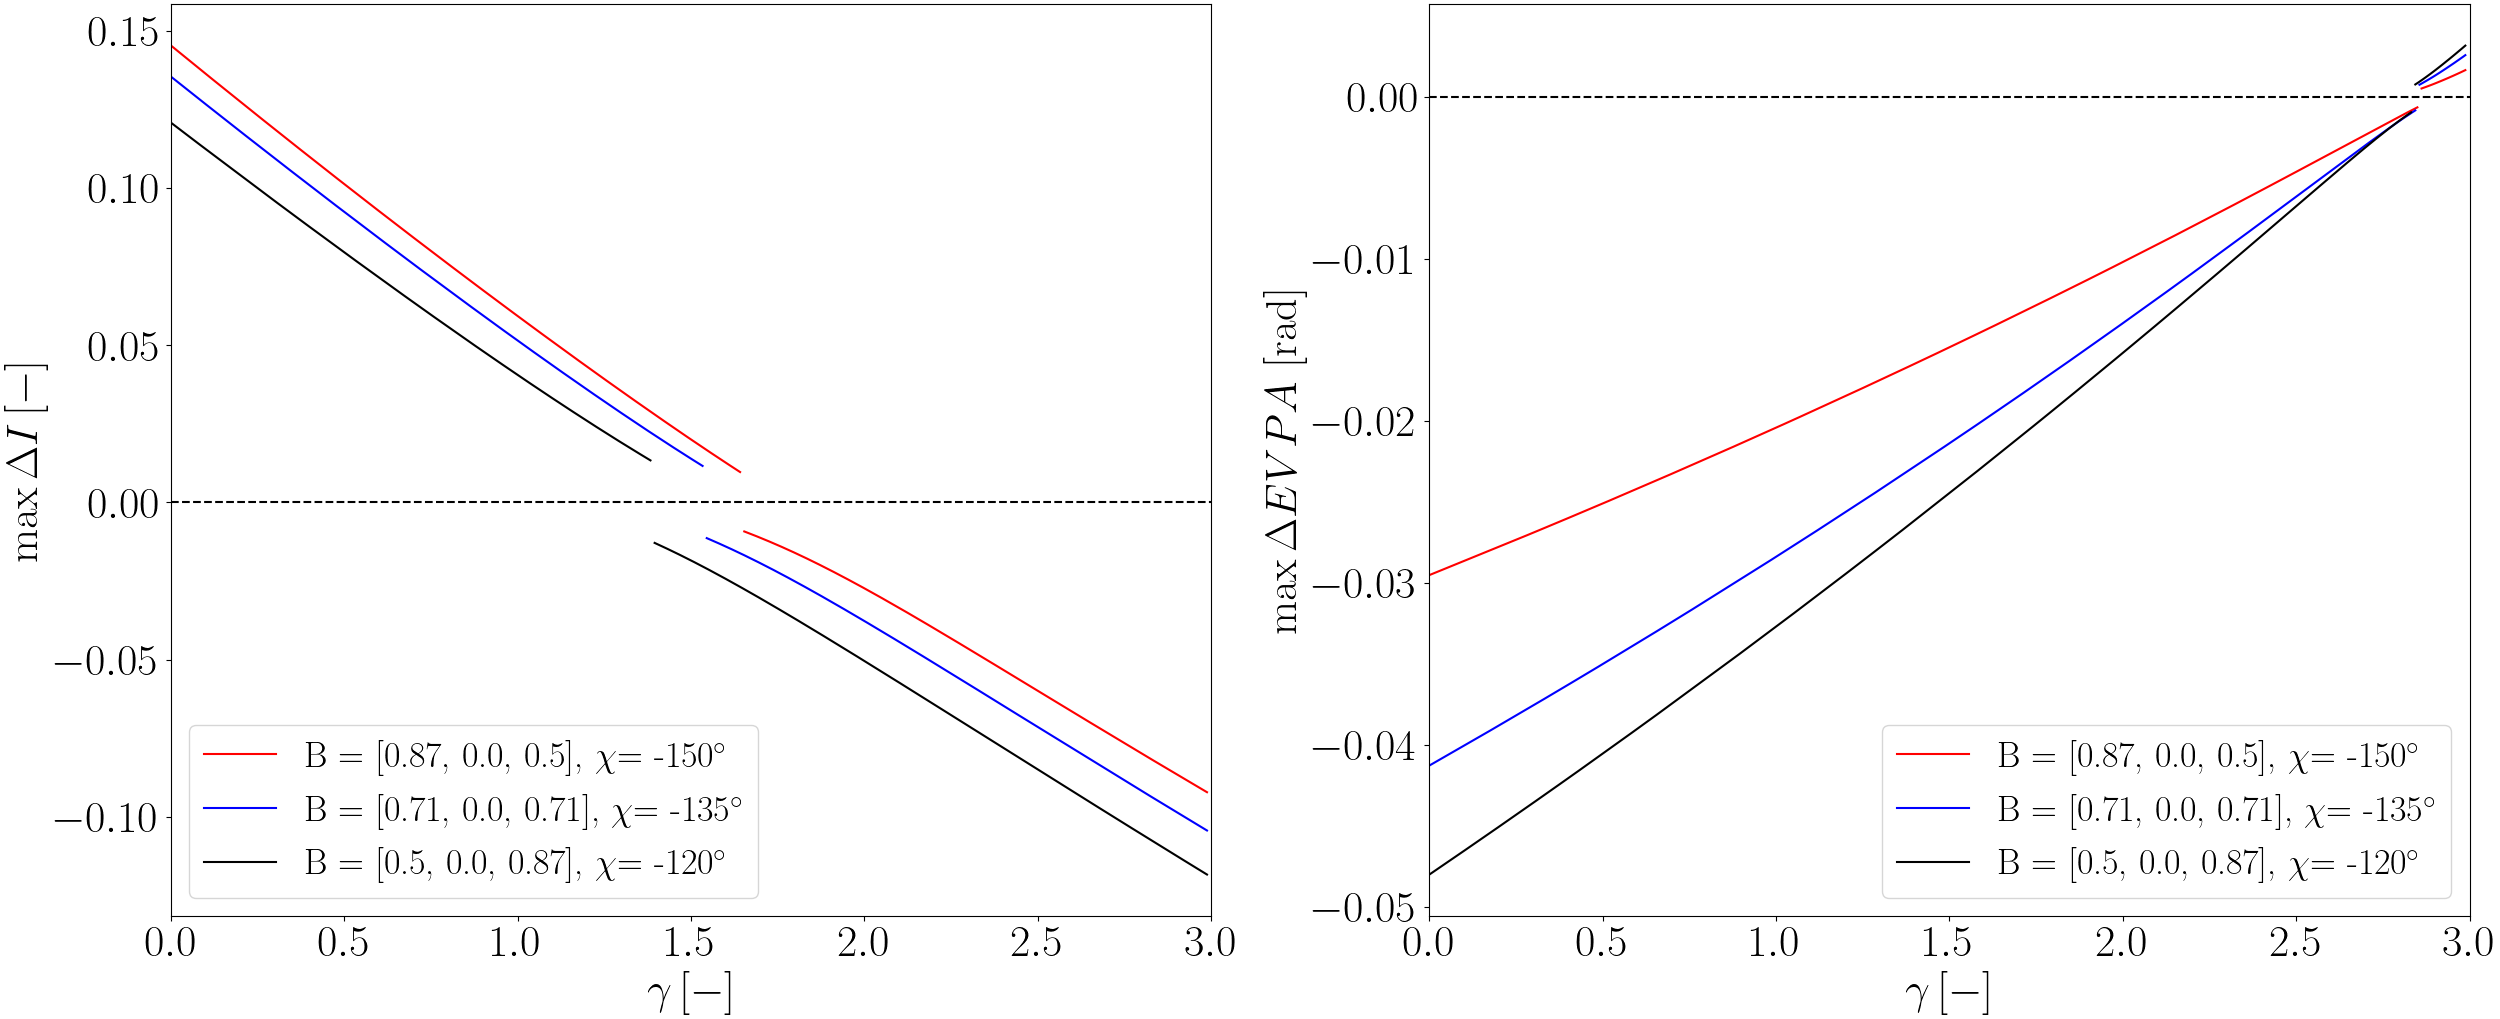
\includegraphics[scale = 0.22]{WH_20_deg_param_sweep.png}
		\caption[Максималното отклонение на поляризираните образи от тип $\{x,y\}\vert_{6M, \text{Schw}}$, за $i = 20\deg$]{Максималното отклонение на поляризираните образи от тип $\{x,y\}\vert_{6M, \text{Schw}}$, за $i = 20\deg$. Отрицателните стойности означават, че съответната величина е по-голяма по модул за черни дупки на Шварцшилд.} 
		\label{WH_max_deviation_20_deg}
\end{figure}
 Резултатите от този анализ са представени в таблица \ref{Deviations_table_20_deg}. Виждаме, че минималните отклонения по интензитет се намират при $\gamma_\text{crit}^{(1)}\approx 1.5$, докато по наклон на поляризационнинят вектор, при $\gamma_\text{crit}^{(2)}\approx 2.85$. Т.е. двете критични стойности на $\gamma$ са значително различни. Също така виждаме, че относителното отклонение в наклона е много малка, дори и за стойности на $\gamma$, далеч от $\gamma_\text{crit}^{(2)}\approx 2.85$. Докато отклоненията по интензитет могат да нарастат до над $20\%$ за $\gamma >> \gamma_\text{crit}^{(1)}$. От това заключваме, че директните образи около пространствено - времеви тунели най-добре възпроизвеждат тези на черни дупки на Шварцшилд при $\gamma = \gamma_\text{crit}^{(1)}$.
\begin{table}[h!]
	\small
	\begin{center}
		\begin{tabular}{||m{7.5em} | m{5em} | m{5em} | m{7em} | m{3em}| m{2em}||} 
			\hline
			Магнитно поле & Величина за минимизиране & \small $\frac{\max\Delta I}{I_\text{Schw}}$ [\%]& \small $\frac{\max\Delta EVPA}{EVPA_{\text{Schw}}}$ [\%] & $\phi$ [rad] & $\gamma_\text{crit}$ \\ [0.5ex] 
			\hline\hline
			\multirow{2}{7.5em}{\small $\vec{B} = [0.5, 0, 0.87]$} & \centering $\Delta I$ & \centering 3.8 & \centering 2.2 &  $0.48\pi$ &  1.39\\ 
																 & \centering $\Delta EVPA$ & \centering 23.0 & \centering 0.3 &  $0.73\pi$ & 2.85\\ 
			\hline
			\multirow{2}{8em}{\small $\vec{B} = [0.71, 0, 0.71]$} & \centering $\Delta I$ & \centering3.6 & \centering1.8 & $0.53\pi$ & 1.54\\ 
																    & \centering $\Delta EVPA$ & \centering23.1 & \centering0.07 & $1.32\pi$ & 2.85 \\ 
			\hline
			\multirow{2}{7.5em}{\small $\vec{B} = [0.87, 0, 0.5]$} & \centering $\Delta I$ & \centering3.3 &\centering 1.1 & $0.53\pi$ & 1.64\\ 
															     & \centering $\Delta EVPA$ & \centering23.4 & \centering0.04 & $0.32\pi$ & 2.86 \\  [1ex] 
			\hline
		\end{tabular}
	\end{center}
	\caption[Отклонения на поляризираните образи от тип $\{x,y\}\vert_{6M, \text{Schw}}$, за $i = 20\deg$, при критичните стойности $\gamma_\text{crit}$]{Отклонения на поляризираните образи от тип $\{x,y\}\vert_{6M, \text{Schw}}$, за $i = 20\deg$, при критичните стойности $\gamma_\text{crit}$. Величините в отношенията на колонки 3 и 4 са пресметнати в една и съща точка от образа.}
	\label{Deviations_table_20_deg}
\end{table}\\

От фигура \ref{WH_max_deviation_20_deg} също можем да оценим и максималните отклонения от Шварцшилд, възможни за този тип метрика. Това се случва при ниски стойности на $\gamma$, независимо от магнитно поле (въпреки, че \emph{големината} на отклонението зависи силно от полето). Виждаме, че при $\gamma = 0$ и $\vec{B} = [0.87, 0, 0.5]$, максималното относително отклонение по интензитет е $\Delta I / I_{\text{Schw}} = 43\%$, докато по наклон е $\Delta EVPA / EVPA_\text{Schw} = 2.3\%$, докато за $\vec{B} = [0.87, 0, 0.5]$ намираме $\Delta I / I_{\text{Schw}} = 28\%$ и $\Delta EVPA / EVPA_\text{Schw} = 3.2\%$.\\

Отклоненията от Шварцшилд за фиксирана стойност на $\gamma$ зависят силно от ориентацията на магнитното поле. За $\gamma < \gamma_\text{crit}^{(1)}$, $\Delta I$ расте с увеличаване на радиалната компонента $B^{(r)}$, докато за $\gamma > \gamma_\text{crit}^{(1)}$ намалява. За разлика от това, $\Delta EVPA$ расте с увеличава на $B^{(r)}$ за всички стойности на $\gamma$. Тези заключения важат и ако разгледаме образи, съответстващи на видимата позиция на $r_s = 4.5$ за Шварцшилд (виж ДОПЪЛНЕНИЕ 4.5 ГРАФИКИ).\\

Като следваща стъпка в изследването си, разгледахме същите образи, но под наблюдателна инклинация $i = 70^\circ$. От фигура \ref{WH_delta_r6_70_deg} виждаме, че по-високата инклинация води до по-силно изразени отклонения на образите. Профилът на отклонение на $EVPA$ има качествено същият характер, с два противоположни по знак пика при $\phi \approx 0$ и $\phi \approx \pi$, но профилът на отклонение на интензитетът е силно различен - ефект който се дължи на много по-силно проявеното Доплерово отместване. Отново забелязваме, че както $\Delta I$, така и $\Delta EVPA$, сменят знака си с промяна на параметъра $\gamma$ - следователно отново съществуват две критични с стойности $\{\gamma_\text{crit}^{(1)}, \gamma_\text{crit}^{(2)}\}$, при които отклонението на образите е най-малко. На фигура \ref{WH_max_deviation_70_deg} отново е начертана максималната стойност на отклоненията като функция на $\gamma$, и в таблица \ref{Deviations_table_70_deg} са обобщени резултатите за отклоненията. \newpage

\begin{figure}[!htb]
	\centering
	\begin{subfigure}{12cm}
		\hspace{-2cm}
		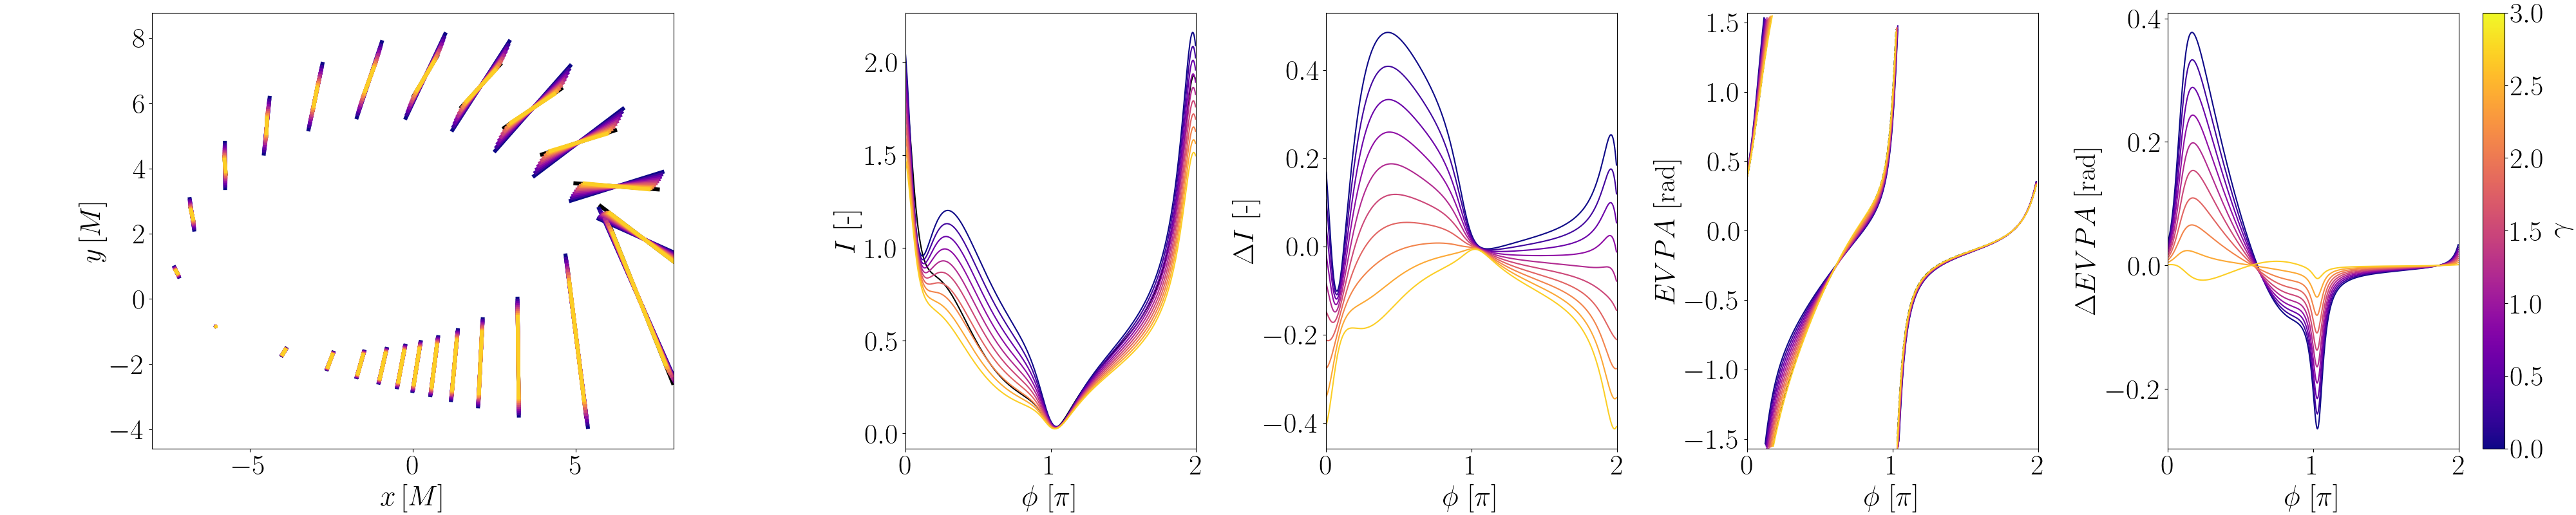
\includegraphics[scale = 0.15]{WH_delta_fig_B_0.5_0.87_0_70_deg_r6.png}
		\caption{$\vec{B} = [0.5, 0, 0.87]$, $\beta = 0.3$, $\chi = -120^\circ$.} 
	\end{subfigure}\\
	\begin{subfigure}{12cm}
		\hspace{-2cm}
		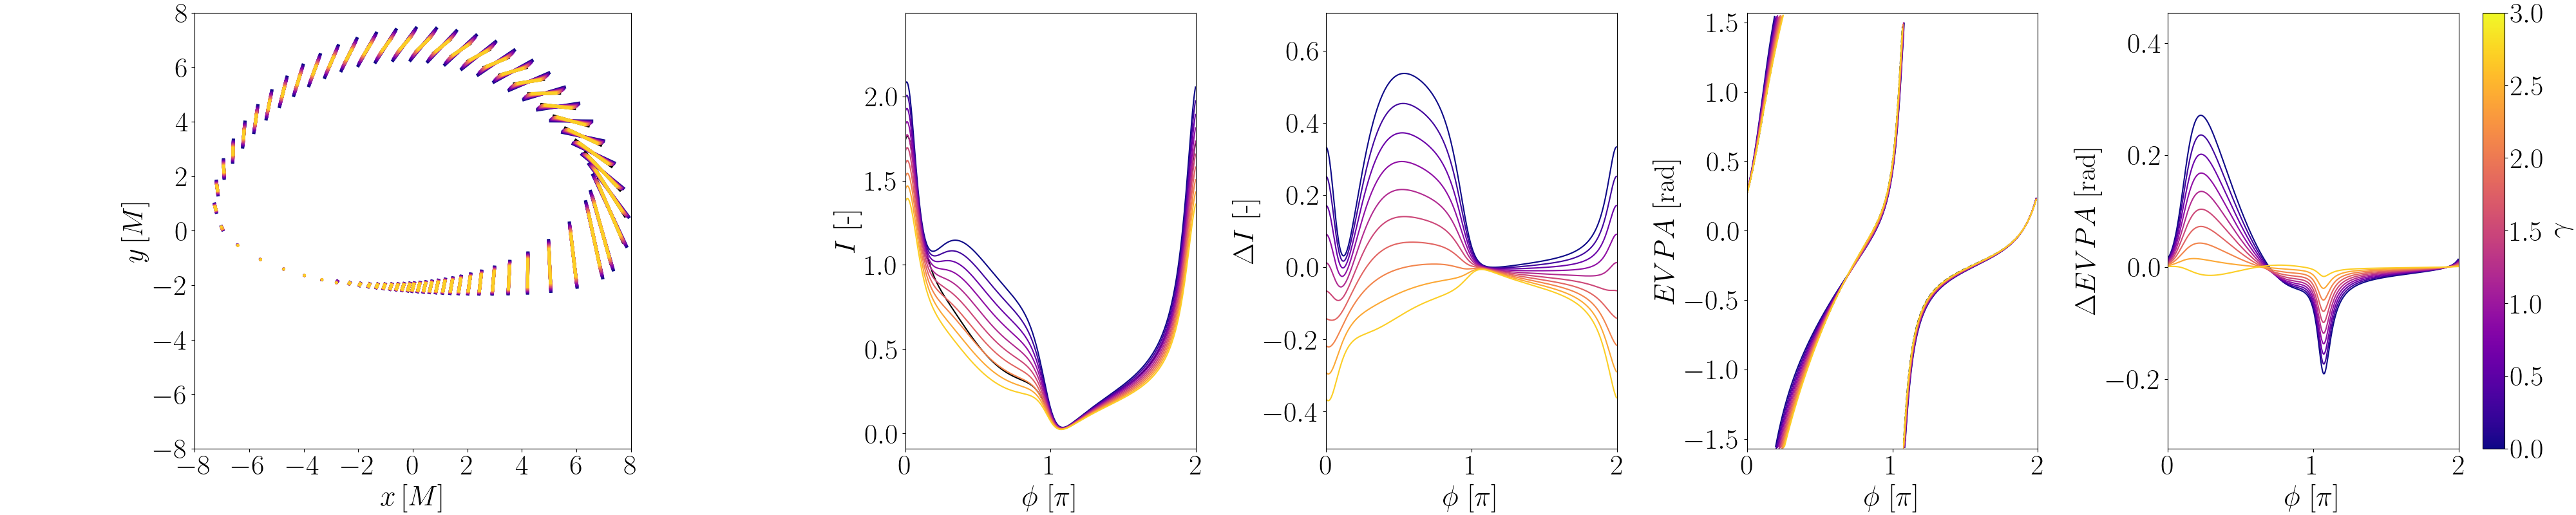
\includegraphics[scale = 0.15]{WH_delta_fig_B_0.71_0.71_0_70_deg_r6.png}
		\caption{$\vec{B} = [0.71, 0, 0.71]$, $\beta = 0.3$, $\chi = -135^\circ$.}
	\end{subfigure}\\
	\begin{subfigure}{12cm}
		\hspace{-2cm}
		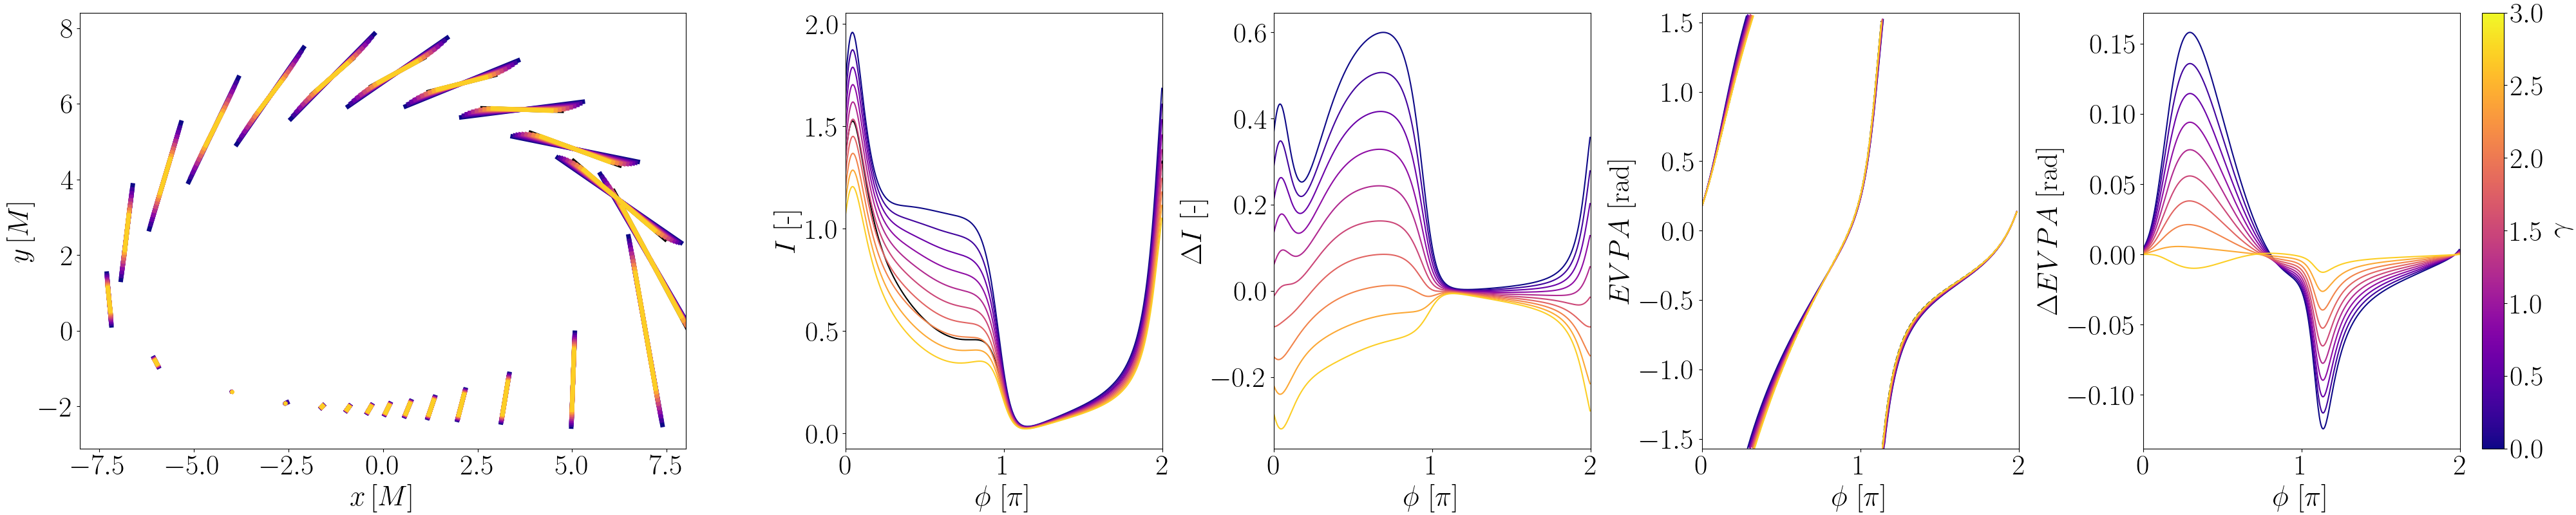
\includegraphics[scale = 0.15]{WH_delta_fig_B_0.87_0.5_0_70_deg_r6.png}
		\caption{$\vec{B} = [0.87, 0, 0.5]$, $\beta = 0.3$, $\chi = -150^\circ$.}
	\end{subfigure}
	\caption[Профили на отклоненията на поляризираните образи oт тип $\{x,y\}\vert_{6M, \text{Schw}}$, за $i = 70\deg$.]{\small Профили на отклоненията на поляризираните образи от тип $\{x,y\}\vert_{6M, \text{Schw}}$, за $i = 70\deg$. Черната крива на $I(\phi)$ съответства на черни дупки на Шварцшилд.} 
	\label{WH_delta_r6_70_deg}
\end{figure}

\begin{figure}[!htb]
	\centering
	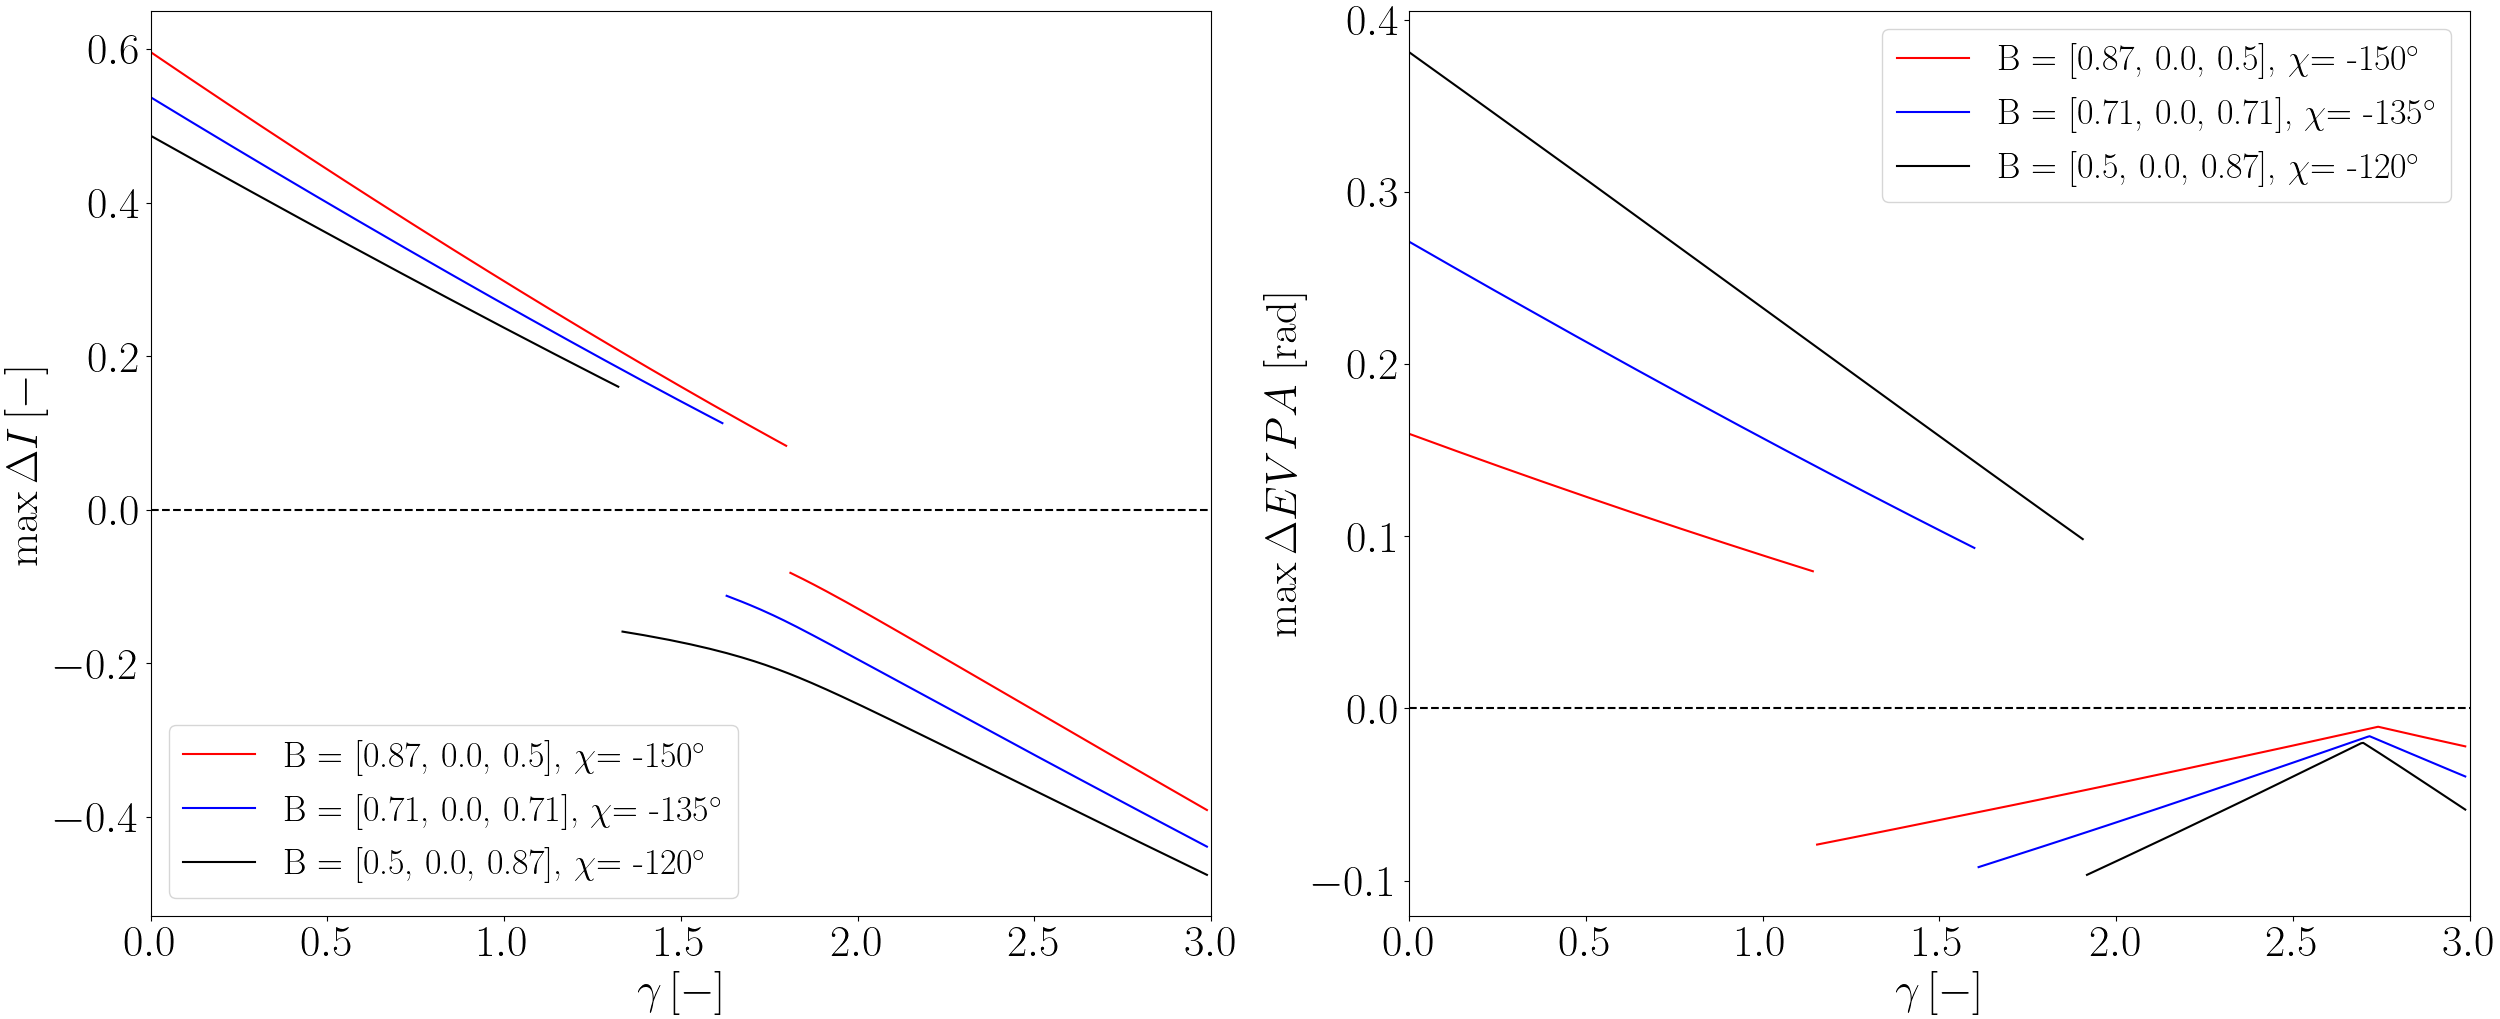
\includegraphics[scale = 0.22]{WH_70_deg_param_sweep.png}
	\caption[Максималното отклонение на директните поляризираните образи от тип $\{x,y\}\vert_{6M, \text{Schw}}$, за $i = 70\deg$]{Максималното отклонение на директните поляризираните образи от тип $\{x,y\}\vert_{6M, \text{Schw}}$, за $i = 70\deg$. Отрицателните стойности означават, че съответната величина е по-голяма по модул за черни дупки на Шварцшилд.} 
	\label{WH_max_deviation_70_deg}
\end{figure}

Виждаме, че минималното отклонение от Шварцшилд расте с увеличаване на инклинацията. Това е така и при неподвижен флуид, тъй като за да формират тези образи, фотоните трябва да се закривят значително повече, и следователно относителното влияние на пространство-времето е по-високо.

\begin{table}[h!]
	\small
	\begin{center}
		\begin{tabular}{||m{7.5em} | m{5em} | m{5em} | m{7em} | m{3em}| m{2em}||} 
			\hline
			Магнитно поле & Величина за минимизиране & \small $\frac{\max\Delta I}{I_\text{Schw}}$ [\%]& \small $\frac{\max\Delta EVPA}{EVPA_{\text{Schw}}}$ [\%] & $\phi$ [rad] & $\gamma_\text{crit}$ \\ [0.5ex] 
			\hline\hline
			\multirow{2}{7.5em}{\small $\vec{B} = [0.5, 0, 0.87]$} & \centering $\Delta I$ & \centering 12.2 & \centering 11.2 &  $0.06\pi$ &  1.33\\ 
			& \centering $\Delta EVPA$ & \centering 21.5 & \centering 1.6 &  $1.04\pi$ & 2.70\\ 
			\hline
			\multirow{2}{8em}{\small $\vec{B} = [0.71, 0, 0.71]$} & \centering $\Delta I$ & \centering 7.3 & \centering 6.3 & $0.06\pi$ & 1.63\\ 
			& \centering $\Delta EVPA$ & \centering 21.3 & \centering 1.3 & $1.08\pi$ & 2.72 \\ 
			\hline
			\multirow{2}{7.5em}{\small $\vec{B} = [0.87, 0, 0.5]$} & \centering $\Delta I$ & \centering 6.3 &\centering 3.6 & $1.98\pi$ & 1.82\\ 
			& \centering $\Delta EVPA$ & \centering 21.5 & \centering 0.9 & $1.14\pi$ & 2.75 \\  [1ex] 
			\hline
		\end{tabular}
	\end{center}
	\caption[Отклонения на поляризираните образи от тип $\{x,y\}\vert_{6M, \text{Schw}}$, за $i = 70\deg$, при критичните стойности $\gamma_\text{crit}$]{Отклонения на поляризираните образи от тип $\{x,y\}\vert_{6M, \text{Schw}}$, за $i = 70\deg$, при критичните стойности $\gamma_\text{crit}$. Величините в отношенията на колонки 3 и 4 са пресметнати в една и съща точка от образа.}
	\label{Deviations_table_70_deg}
\end{table}

Най-голямото отклонение отново е при $\gamma =0$. Тогава за магнитно поле $\vec{B} = [0.87, 0, 0.5]$ имаме максимално относително отклонение в интензитета $\Delta I / I_\text{Schw} = 128\%$, докато за наклона  $\Delta EVPA / EVPA_\text{Schw} = 11\%$.

\subsubsection{Поляризация на индиректните образи}
Сега нека обърнем внимание на индирертните образи - по-конкретно на случая за $n=1$. Те са представени на фигура \ref{WH_pol_eq_field_n1}. Виждаме, че отново качественият характер с сходен със Шварцшилд, но видимият радиус на образа, за разлика от директният случай, се мени силно с $\gamma$. Това води до важно следствие: Докато директни образи от тип $\{x,y\}\vert_{X, \text{Schw}}$ съществуваха за всички стойности на $\gamma$, за индиректните това не е така. Причината е, че поради силният ефект на лещата, те се намират в много близка околност до сянката на тунела, чиито радиус зависи силно от параметъра $\gamma$ (виж фигури \ref{WH_gamma_70_deg} и \ref{WH_gamma_20_deg}).\\

За да изследваме при какви стойности на $\gamma$ можем да намерим образи от тип $\{x,y\}\vert_{X, \text{Schw}}$, нека погледнем фигура \ref{WH_n1_overlap}. Начертани са кривите $r_\text{img, in}(\phi)$ и $r_\text{img, out}(\phi)$$^1$ за екваториален диск с граници $r_\text{in} = 4.5M$, $r_\text{out} = 500M$, при избрани стойности на $\gamma$. Съществуването на образи от тип $\{x,y\}\vert_{X, \text{Schw}}$ е възможно само ако е изпълнено поне едно от следните две условия:

\lfoot{\noindent\makebox[\linewidth]{\rule{\textwidth}{0.4pt}}
	\small$^1$ С величината $r_{\text{img}}(\phi) = \sqrt{x^2(\phi) + y^2(\phi)}$ бележим радиусът на образа, при ъгловата позиция $\phi$.}

\begin{subequations}
	\begin{equation}
		r_\text{img, in}^{\text{(Schw)}}(\phi) \le r_\text{img, out}^{\text{(WH)}}(\phi) \le r_\text{img, out}^{\text{(Schw)}}(\phi)\,\,\, \forall\phi\in[0,2\pi]
	\end{equation}
	\begin{equation}
		r_\text{img, in}^{\text{(Schw)}}(\phi) \le r_\text{img, in}^{\text{(WH)}}(\phi) \le r_\text{img, out}^{\text{(Schw)}}(\phi)\,\,\, \forall\phi\in[0,2\pi]
	\end{equation}
\end{subequations}
\newpage
\begin{figure}[!htb]
	\hspace{-0.2cm}
	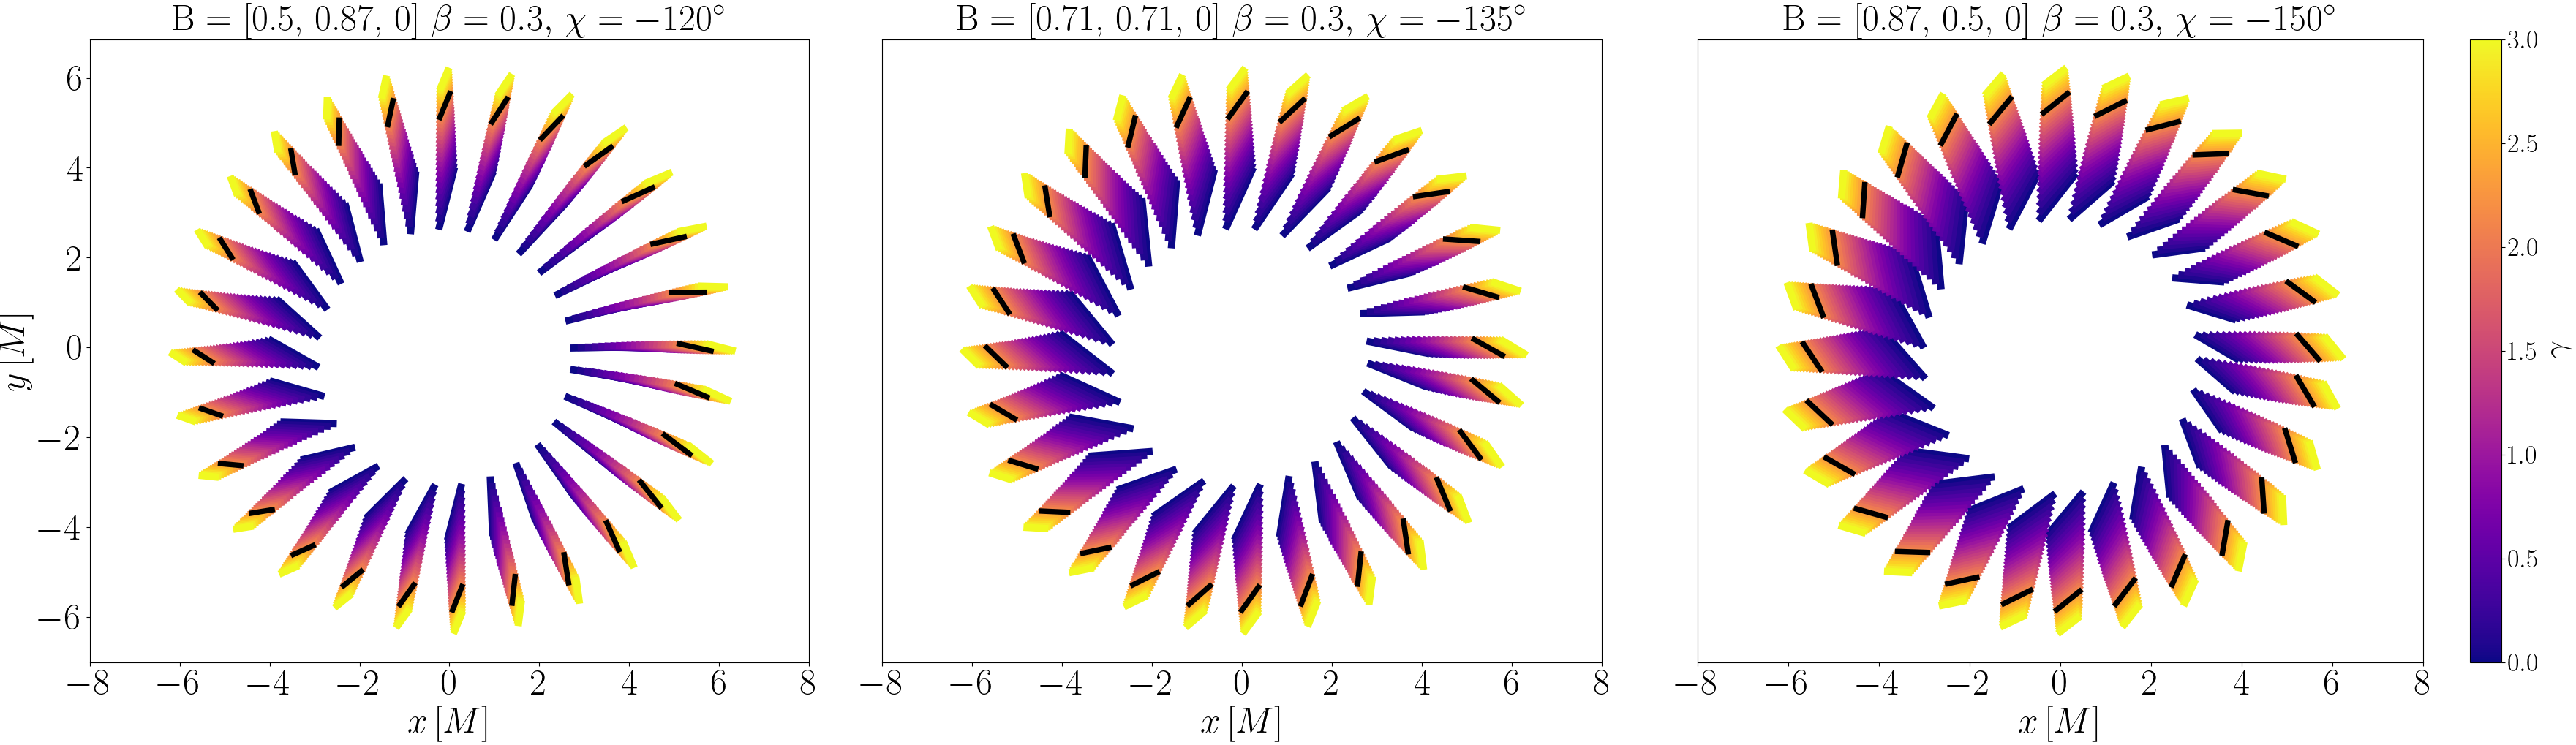
\includegraphics[scale = 0.17]{WH_alpha_Eq_Field_n1.png}
	\caption[Поляризирани $n=1$ образи около пространствено - времеви тунели за екваториално магнитно поле.]{\small Построените $n=1$ поляризирани образи на орбитата $r_s = 6M$ около пространствено - времеви тунели за екваториално магнитно поле и $\gamma \in[0,3]$ и $i = 20^\circ$. Черните линии съответстват на черна дупка на Шварцшилд.} 
	\label{WH_pol_eq_field_n1}
\end{figure}

\lfoot{}
Както можем да видим от фигура \ref{WH_n1_overlap}, удовлетворяването на поне едно от условията (7.28) е възможно само за  $1.8 \lessapprox \gamma \lessapprox 2.7$. Следователно ще се фокусираме само върху тези стойности. Имайки предвид морфологичната прилика на индиректните образи на пространствено-времевия тунел тези на Шварцшилд (фигура \ref{WH_pol_eq_field_n1}), отново извършваме количествено сравнение на образите от тип $\{x,y\}\vert_{6M, \text{Schw}}$ - показано на фигура \ref{WH_delta_r6_20_deg_n1}.\\

\begin{minipage}{16em}
	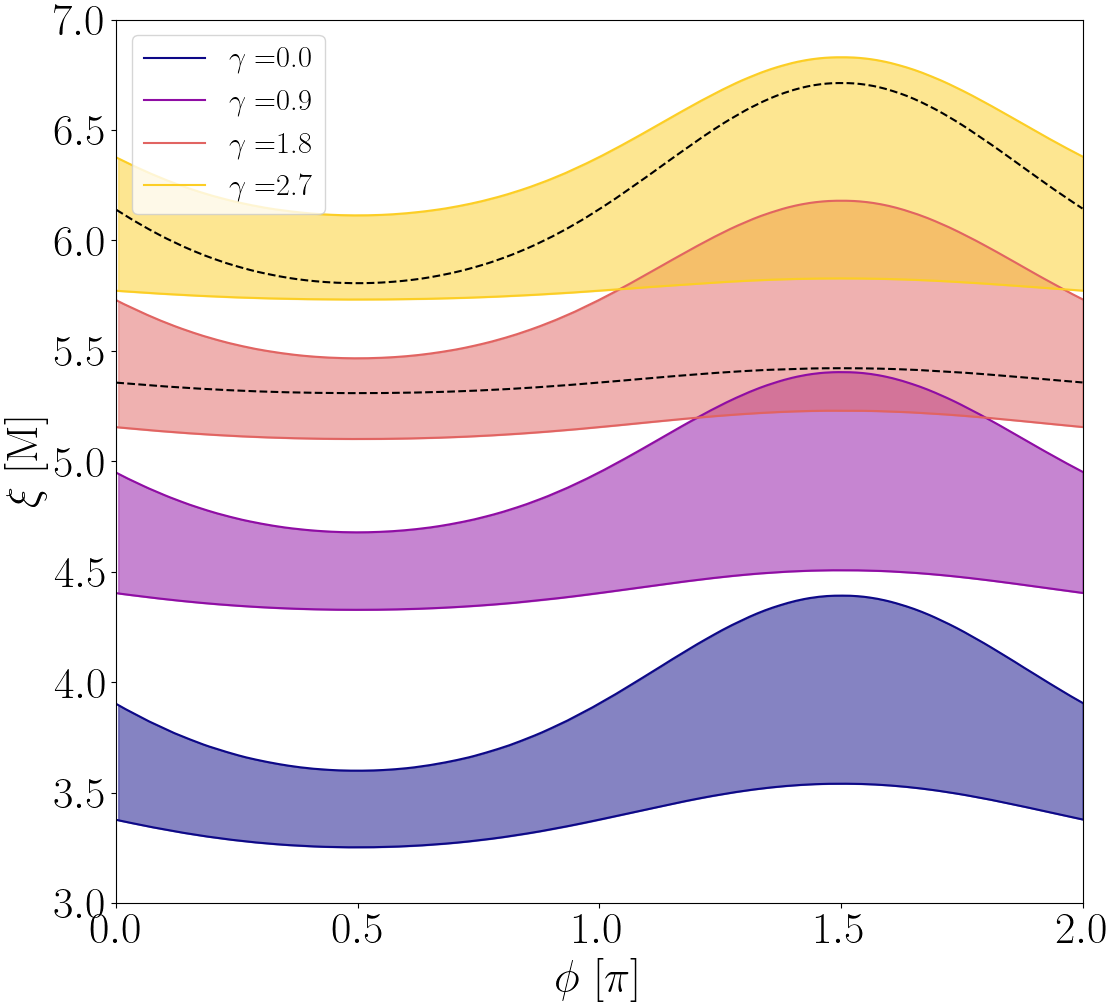
\includegraphics[scale = 0.22]{WH_indirect_overlap_grapth.png}
	\captionof{figure}[Диаграма на формиране на образи от тип $\{x,y\}\vert_{X, \text{Schw}}$ ]{Диаграма на формиране на образи от тип $\{x,y\}\vert_{X, \text{Schw}}$. Tя показва графично зоните, в които е изпълнено (7.28), за избрани стойности на $\gamma$. Черните пунктири съответстват на черни дупки на Шварцшилд. Виждаме, че приблизителният диапазон на съществуване е $1.8 \lessapprox \gamma \lessapprox 2.7$.} 
	\label{WH_n1_overlap}
\end{minipage}\,\,
\begin{minipage}{20em}
	Виждаме, че силният ефект на гравитационната леща води до много по-значителни отклонения в образите. Максималното относително отклонение в интензитетът достига $\max \Delta I / I_{\text{Schw}} = 650\%$ за магнитно поле $\vec{B} = [0.5, 0, 0.87]$ при $\gamma = 1.78$. За разлика от директните образи наблюдаваме, че $\max\Delta I$ расте с \emph{намаляването} на радиалната компонента на магнитното поле, докато $\max\Delta EVPA$ показва обратният характер. Друг важен белег който наблюдаваме е, че разпределението на интензитета се измества към горната част на образа $\phi = \pi / 2$ с намаляване на $\gamma$, докато при $\gamma = 1.96$ се намира значително по-близко до максимума на Шварцшилд $\phi \approx 0 $.
\end{minipage}

\newpage

На фигура \ref{WH_max_deviation_20_deg_n1} можем да видим поведението на максималните отклонения.

\begin{figure}[!htb]
	\centering
	\begin{subfigure}{12cm}
		\hspace{-0.5cm}
		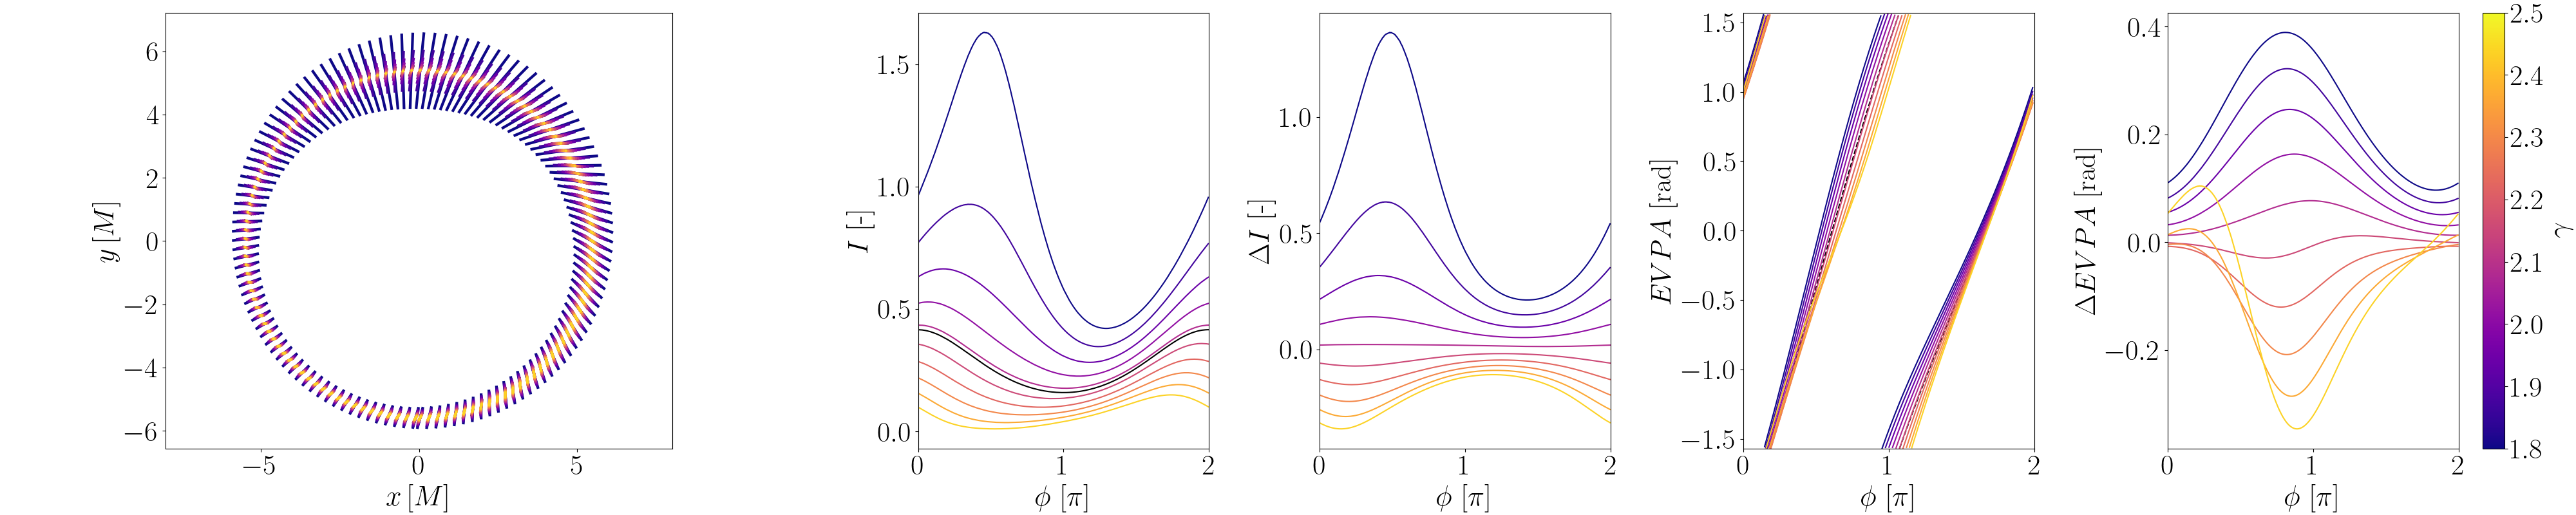
\includegraphics[scale = 0.13]{WH_delta_fig_B_0.5_0.87_0_20_deg_r6_n1.png}
		\caption{$\vec{B} = [0.5, 0, 0.87]$, $\beta = 0.3$, $\chi = -120^\circ$.} 
	\end{subfigure}\\
	\begin{subfigure}{12cm}
		\hspace{-0.5cm}
		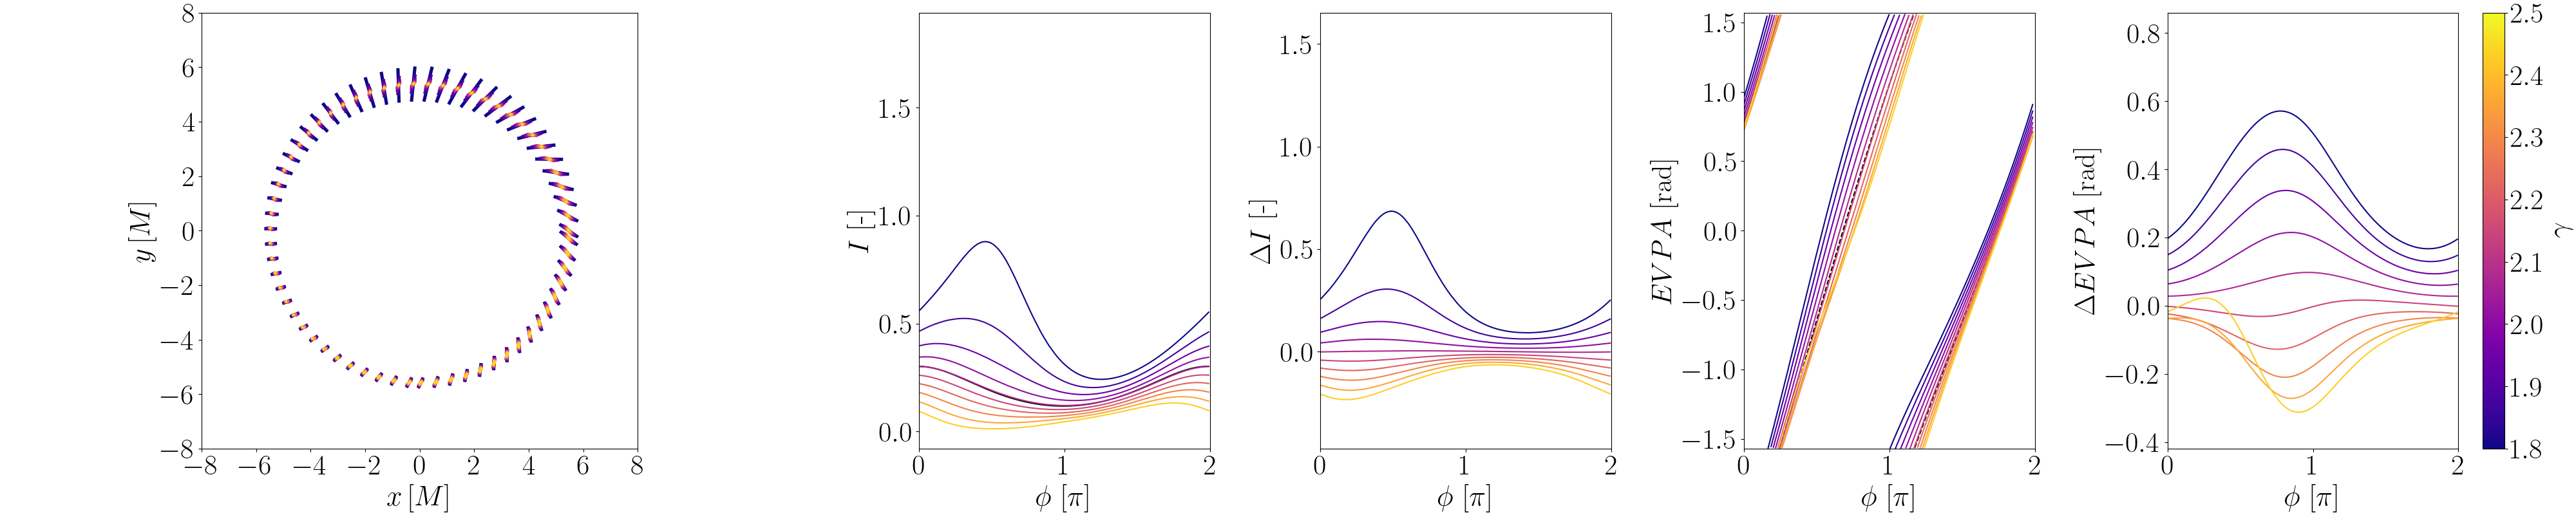
\includegraphics[scale = 0.13]{WH_delta_fig_B_0.71_0.71_0_20_deg_r6_n1.png}
		\caption{$\vec{B} = [0.71, 0, 0.71]$, $\beta = 0.3$, $\chi = -135^\circ$.}
	\end{subfigure}\\
	\begin{subfigure}{12cm}
		\hspace{-0.5cm}
		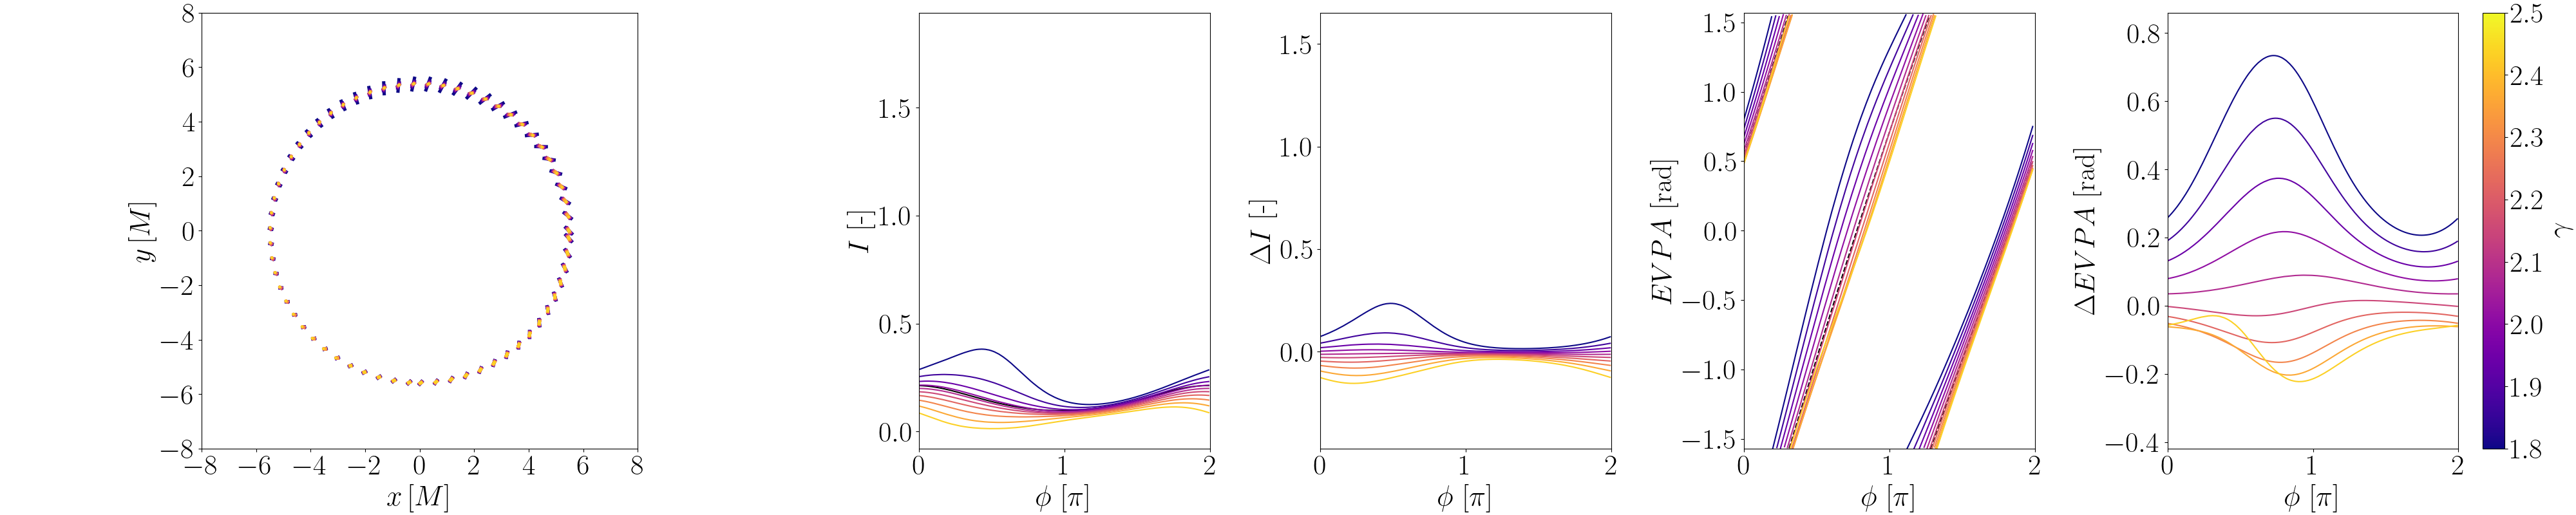
\includegraphics[scale = 0.13]{WH_delta_fig_B_0.87_0.5_0_20_deg_r6_n1.png}
		\caption{$\vec{B} = [0.87, 0, 0.5]$, $\beta = 0.3$, $\chi = -150^\circ$.}
	\end{subfigure}
	\caption[Профили на отклоненията на $n=1$ поляризираните образи oт тип $\{x,y\}\vert_{6M, \text{Schw}}$, за $i = 20\deg$.]{\small Профили на отклоненията на $n=1$ поляризираните образи от тип $\{x,y\}\vert_{6M, \text{Schw}}$, за $i = 20\deg$. Черната крива на $I(\phi)$ съответства на черни дупки на Шварцшилд.} 
	\label{WH_delta_r6_20_deg_n1}
\end{figure}

\begin{figure}[!htb]
	\centering
	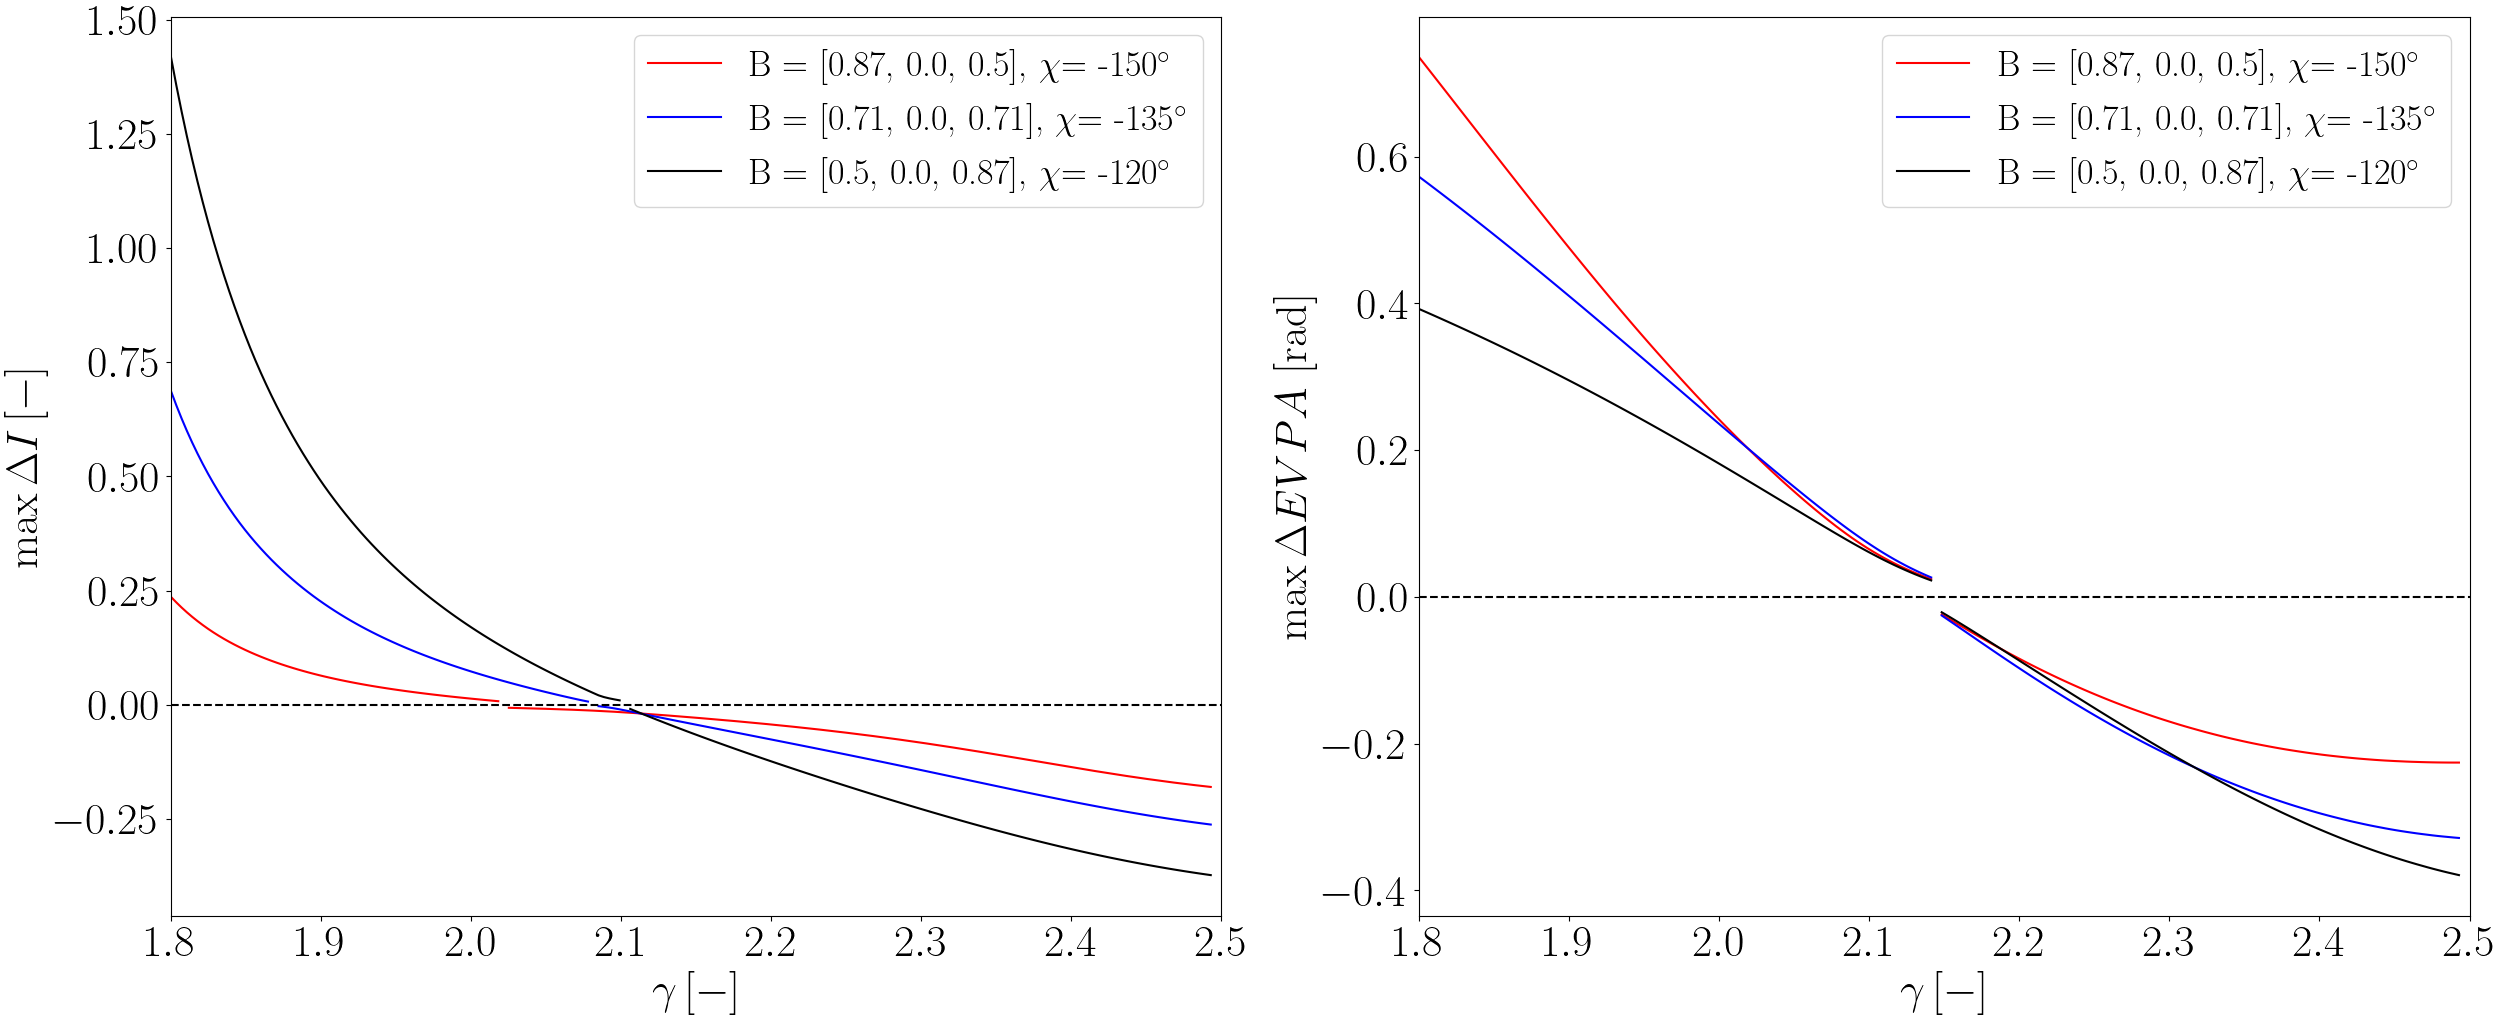
\includegraphics[scale = 0.25]{WH_20_deg_param_sweep_n1.png}
	\caption[Максималното отклонение на $n=1$ поляризираните образи от тип $\{x,y\}\vert_{6M, \text{Schw}}$, за $i = 20\deg$]{Максималното отклонение на $n=1$ поляризираните образи от тип $\{x,y\}\vert_{6M, \text{Schw}}$, за $i = 20\deg$.} 
	\label{WH_max_deviation_20_deg_n1}
\end{figure}
\newpage

\subsubsection{Заключение}

До тук изследвахме линейно поляризираните образи на тънък екваториален акреционен диск около определен клас пространствено - времеви тунели. Целта ни е да дадем оценка за влиянието на природата на пространство - времето върху наблюдаваната поляризация. С помощта на на опростен аналитичен модел на излъчването, и численият код Mjølnir, симулирахме наблюдателните величини на образите в това пространство-време. Фокусирахме се върху набора физични параметри, които произвеждат образи, морфологично сходни на резултатите представени в \cite{EHT_M87_I} - \cite{EHT_M87_VIII}. Поради тази причина изключихме вертикални магнитни полета от разглежданията си.\\

Първо разгледахме директните образи при ниски инклинации. Показахме, че те \emph{не} показват морфологично нови свойства, поради което се фокусирахме върху количествени оценки на отклоненията им спрямо черни дупки на Шварцшилд. Показваме, че за всички разгледани стойности на $\gamma$, относителното отклонение по интензитет не надвишава $\approx 43\%$, а по наклон на поляризационният вектор - не повече от $3.8\%$. Също показахме, че с подобаващ избор на $\gamma$, поляризираните образи от тунела могат да възпроизведат тези на Шварцшилд с точност $4\%$ относително отклонение по всички наблюдаеми величини. \\

Увеличавайки инклинацията виждаме, че отклоненията растат - за наклона на вектора на поляризацията могат да достигнат $25\%$, но морфологията им остава качествено същата като при Шварцшилд. На базата на това можем да заключим следното:\\

\emph{Директните образи на излъчващата среда се влияят слабо от природата на пространство времето. Доминантният физически фактор, определящ тяхното свойство е магнитното поле.}\\

След това разгледахме индиректните образи с $n = 1$. Показваме, че при тях относителните отклонения в интензитета спрямо Шварцшилд могат да достигнат над 6 пъти, докато в наклона до $50\%$. Наблюдаваме също така и морфологична разлика при по-ниските стойности на $\gamma$ - видимият максимум на интензитета се измества в горната част на образа $\phi\approx\pi / 2$. От това заключваме следното:\\

\emph{Индиректните образи се влияят силно както от магнитното поле, така и от природата на пространство-времето.}\\

Следователно можем да предложим следният "алгоритъм"$\,$ за груба оценка на самосъгласуваността на модела на централният обект и излъчващата среда, на база съгласуването на образите с $n = 0$ и $n = 1$. Предполагайки, че можем оптически да ги разделим при наблюдавате, можем да използваме образите с $n = 0$, за оценка на локалното магнитно поле. Наблюденията на M87$^*$ и Sgr A$^*$ показват, че може да очакваме "подредена"$\,$ структура на полето (т.е. с малка турбуленция). Имайки така оценка, можем да я използваме за пресмятането на поляризацията на образите с $n = 1$, които тогава да сравним с наблюдаваните. Ако намерим отклонения в стойността на интензитета, или в ъгловата позиция на максимума му, подобни на тези показани във фигура \ref{WH_delta_r6_20_deg_n1}, можем да съдим, че физичната ни картинка на излъчващата среда и компактният обект не са самосъгласувани. Това е далеч от силен критерии, по който да се съди за природата на компактният обект, но може да служи като наблюдателен белег за несъгласуваност в цялостният ин модел, описващ наблюденията.\\

Тук възниква въпроса до каква степен е възможно да се отделят образите $n = 0$ и $n = 1$ от всички останали в реалните наблюдения. Мотивирани от този въпрос, както и възможността да наблюдаваме екзотичните образи от глава 6, в глава 8 ще симулираме реални наблюдения на описните в глава 5 метрики, с помощта на софтуерният пакет ehtim$^{18}$.

\subsection{Поляризация от голи сингуларности на Джанис - Нюман - Уиникър}

Като допълнение към изследванията ни в 7.2, тук ще разгледаме дали заключенията, които направихме за пространствено-времевите тунели могат да се обобщят и за голи сингулярности. Целим да разберем следното:\\

\textbf{1)} Дали резултатите, представени в 7.2 са специфични за разглежданото пространство-време, или заключенията там могат да се обобщат за други метрики?\\

\textbf{2)} Дали голите сингулярности биха проявили специфични морфологични отклонения на техните поляризирани образи такива, че \emph{качествено} се разграничат, спрямо тези на пространствено-времевия тунел?\\

Анализът ни тук ще протече през аналогични стъпки на 7.2. Подобно изследване е вече правено (въпреки, че не в контекста на сравняване на отклоненията с 3та метрика) за решението на Гаус-Боне \cite{Qin2021}, поради което ние избираме да се фокусираме върху решението на Джанис-Нюман-Уиникър за параметъра $\gamma \in [0.53, 1)$. Този интервал е избран на база \cite{Kocherlakota2021}  където е показано, че за $\gamma < 0.53$, решението не би могло да опише видимата сянка на М87$^*$. 

\subsubsection{Поляризация на директните образи}

Нека първо изследваме дали решението на Джанис-Нюман-Уиникър може да промени съществено морфологията на директните поляризирани орбити при наличието на вертикално магнитно поле. На фигура \ref{JNW_pol_vert_field} са показани поляризираните образи на орбитите $r_s = \{4.5M,6M\}$ за набор от стойности на скаларният параметър в интервала $\gamma\in[0.53,1)$.\\

Виждаме качествено същото поведение като фигура \ref{WH_pol_vert_field}. Т.е. морфологията на вектора на поляризацията се запазва и той единствено се отмества навътре и намалява по големина с намаляването на скаларният параметър $\gamma$. Тогава можем да заключим, че:\\

\emph{И в случая на голи сингулярности, ефектът на лещата при директните образи не е достатъчно различен от черни дупки на Шварцшилд, за да остави морфологичен отпечатък върху поляризацията на тези образи при наличието на вертикално магнитно поле.}

\begin{figure}[!htb]
	\centering
	\begin{subfigure}{7cm}
		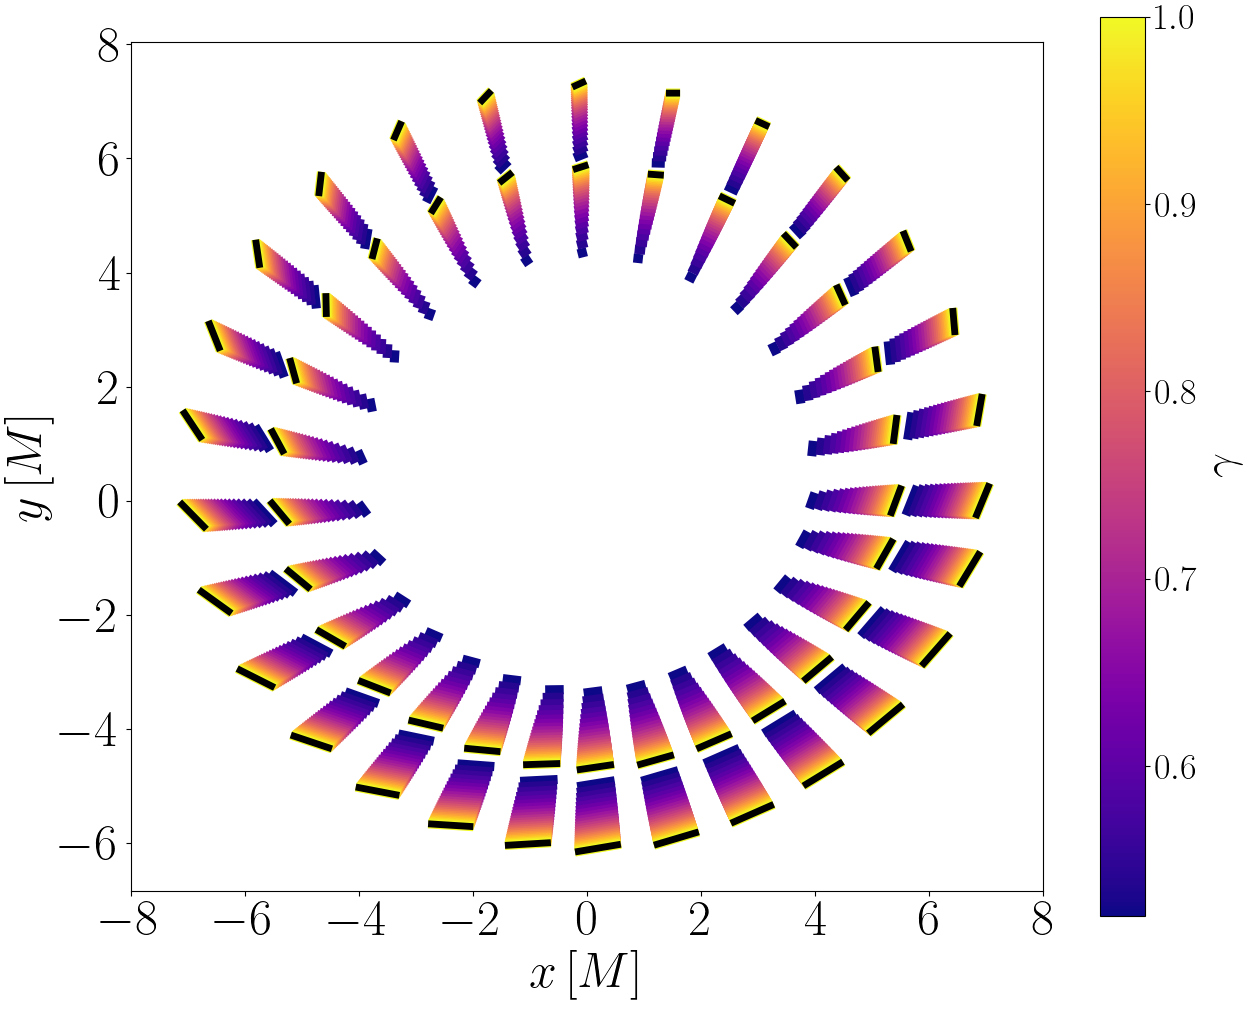
\includegraphics[scale = 0.2]{JNW_alpha_Vert_Field.png}
		\caption{$\vec{B} = [0, 1, 0]$, $\beta = 0.3$, $\chi = -150^\circ$.} 
	\end{subfigure}
	\begin{subfigure}{7cm}
		\hspace{1cm}
		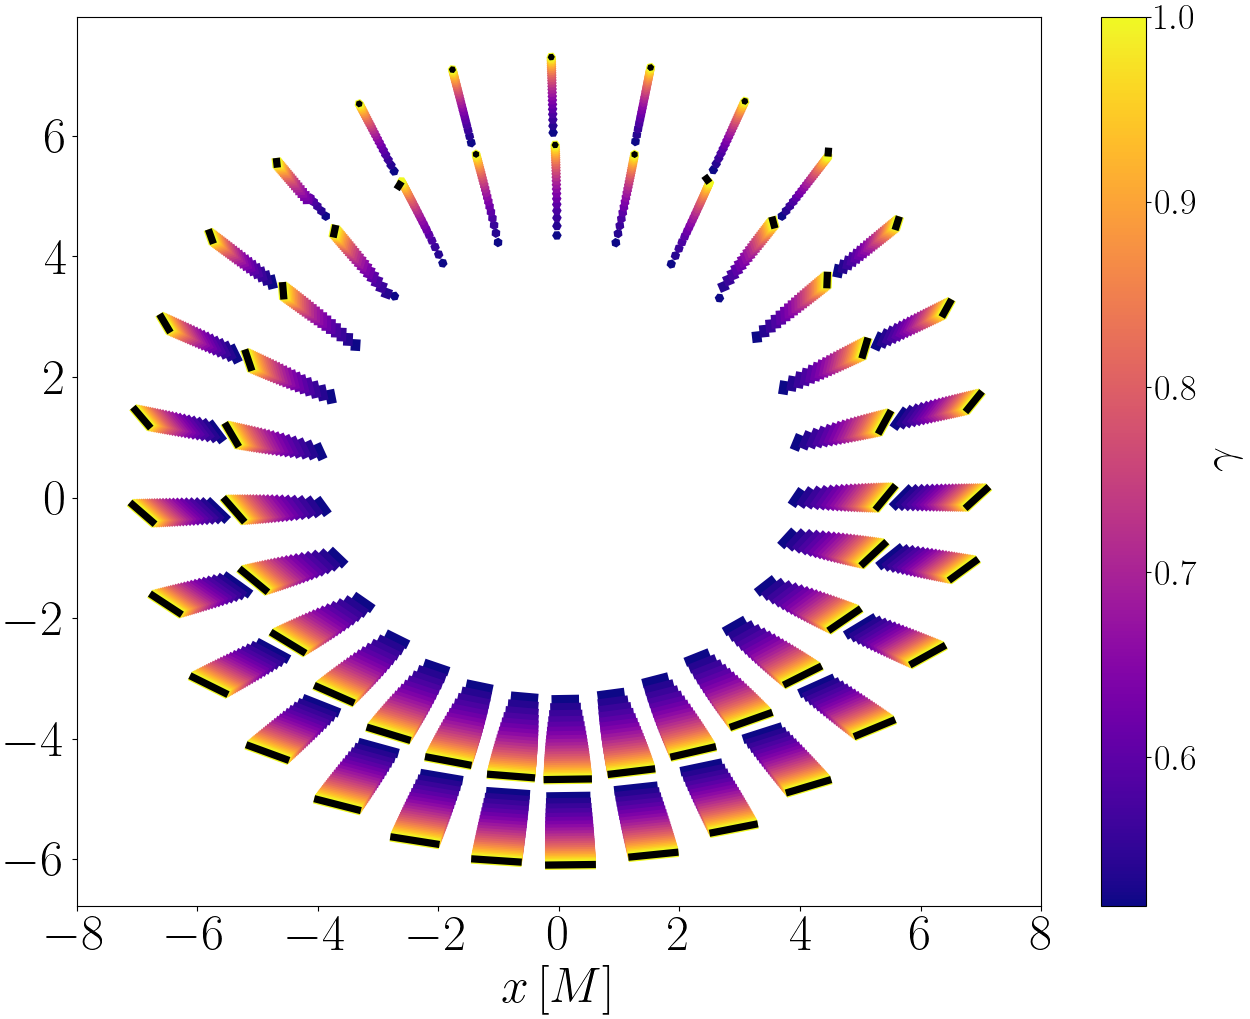
\includegraphics[scale = 0.2]{JNW_alpha_Vert_Field_beta_zero.png}
		\caption{$\vec{B} = [0, 1, 0]$, $\beta = 0$, $\chi = -150^\circ$.}
	\end{subfigure}
	\caption[Поляризирани образи около пространствено - времеви тунели за вертикално магнитно поле.]{\small Построените поляризирани образи на орбитите $r_s = 6M$, $r_s = 4.5M$ около пространствено - времеви тунели за вертикално магнитно поле и $\gamma \in[0,3]$ и $i = 20^\circ$. Черните линии съответстват на черна дупка на Шварцшилд.} 
	\label{JNW_pol_vert_field}
\end{figure}

Имайки това заключение, отново избираме да се фокусираме само върху екваториални магнитни полета. На фигура \ref{JNW_pol_eq_field} показваме същите орбити при $i = 20^\circ$ за 3 конфигурации на магнитното поле.\\

\begin{figure}[!htb]
	\centering
	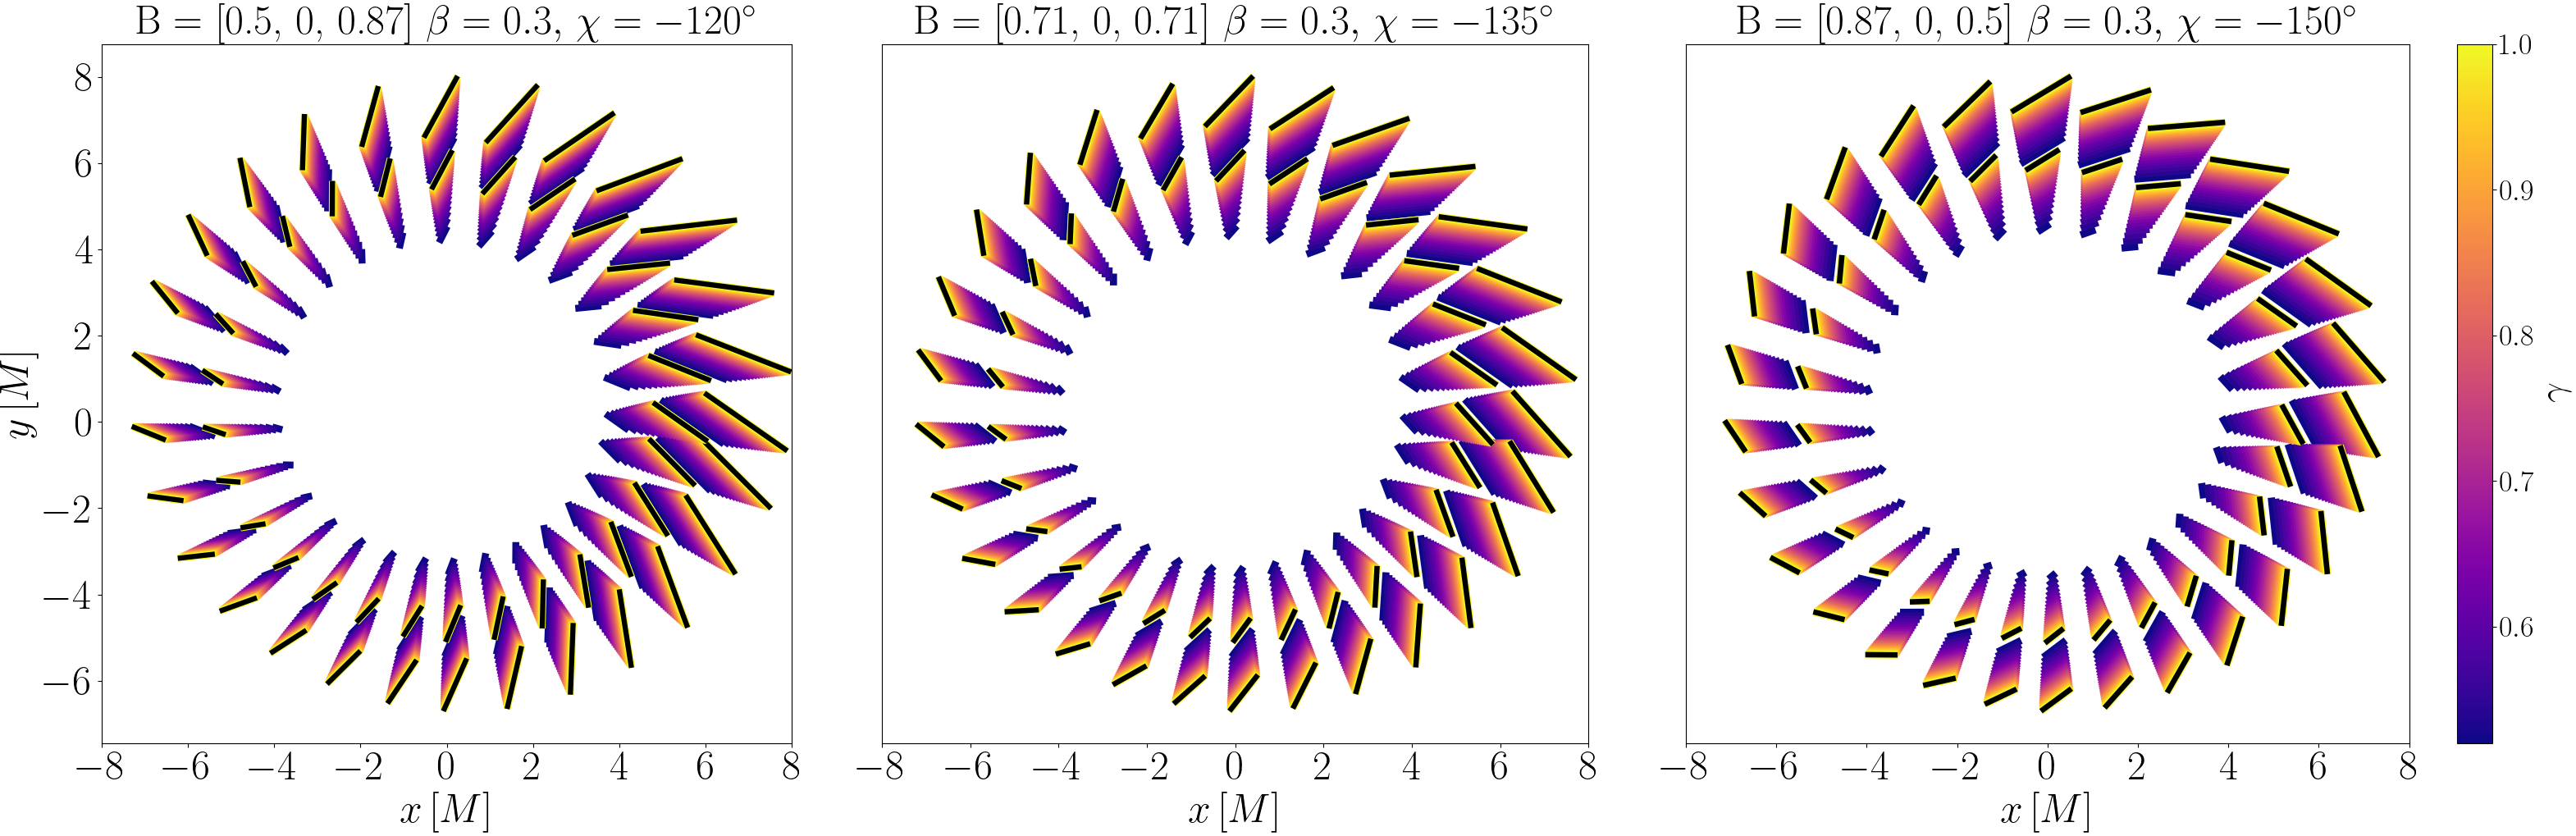
\includegraphics[scale = 0.18]{JNW_alpha_Eq_Field.png}
	\caption[Поляризирани образи около гола сингулярност на Джанис-Нюман-Уиникър за различни екваториални магнитни полета.]{\small Построените поляризирани образи на орбитите $r_s = 6M$, $r_s = 4.5M$ около гола сингулярност на Джанис-Нюман-Уиникър за различни екваториални магнитни полета и $\gamma \in[0.53,1)$ и $i = 20^\circ$. Стойността $\gamma = 1$ съответства на черна дупка на Шварцшилд.} 
	\label{JNW_pol_eq_field}
\end{figure}

Подобно на фигура \ref{WH_pol_eq_field} за  тунела, качественото поведение на вектора на поляризацията при тази гола сингулярност следва това на Шварцшилд. Най-съществената разлика остава различната степен на фокусировка от ефекта на лещата, отговорен за видимото изместване на образите, и различната сила на червеното отместване, отговорно за намаляването на големината на поляризационните вектори. От тук следва, че първоначалното ни заключение за директните образи при пространствено-времевите тунели, също важат и за голи сингулярности, а именно:\\

\emph{Директните образи на голи сингуларности се влияят слабо от природата на пространство-времето, и следователно отклоненията им спрямо черни дупки на Шварцшилд са само количествени.}\\

Разглеждаме подробно тези отклонения при ниски инклинации на фигура \ref{JNW_delta_r6_20_deg}.

\begin{figure}[!htb]
	\centering
	\begin{subfigure}{12cm}
		\hspace{-0.25cm}
		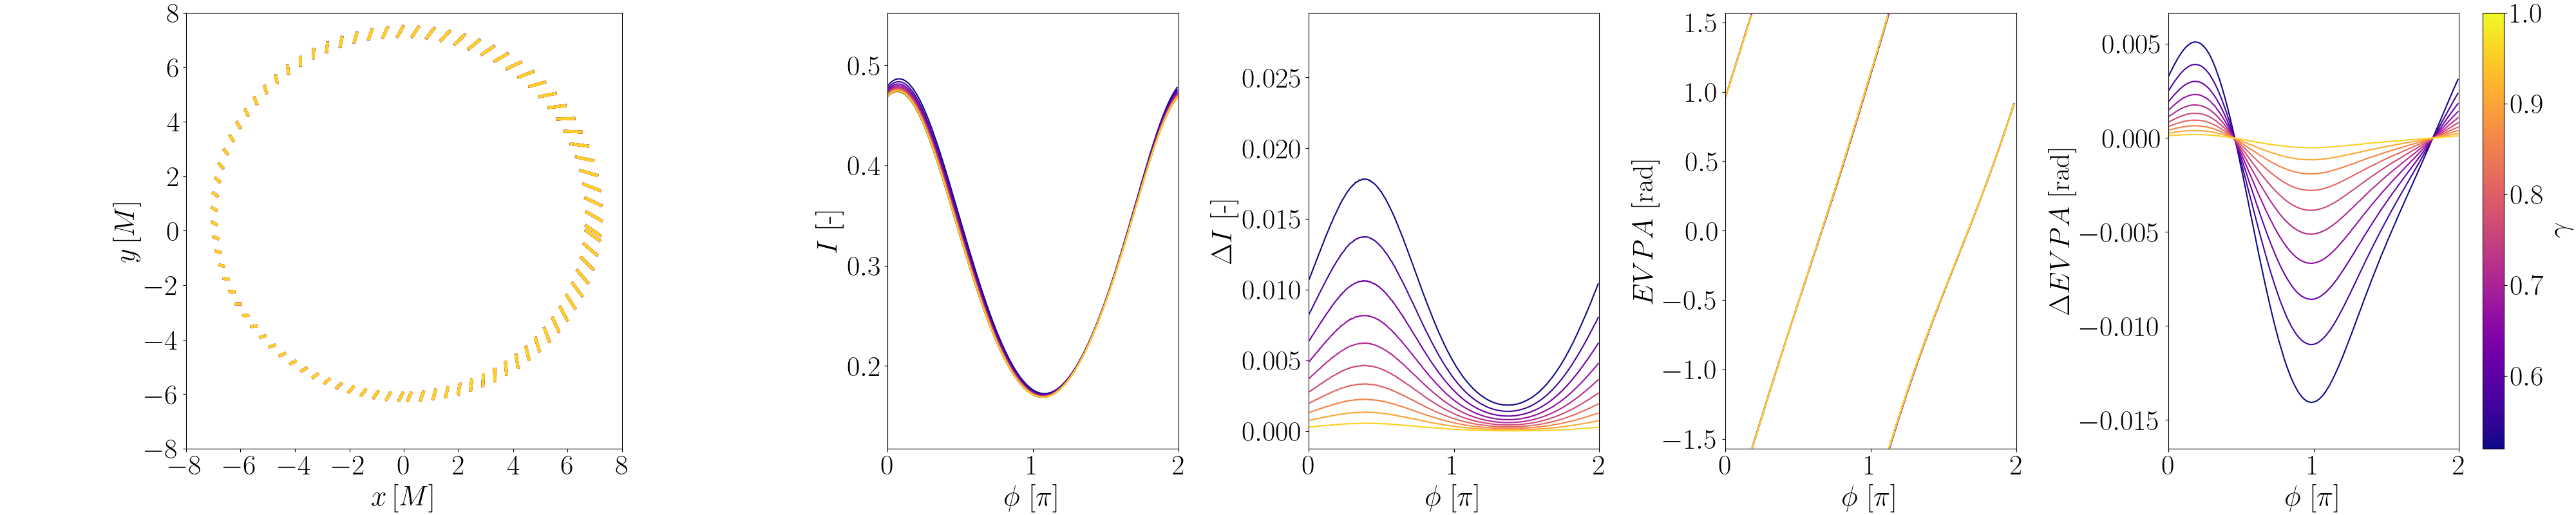
\includegraphics[scale = 0.13]{JNW_delta_figs_B_0.5_0.0_0.87_20_deg_direct.png}
		\caption{$\vec{B} = [0.5, 0, 0.87]$, $\beta = 0.3$, $\chi = -120^\circ$.}
	\end{subfigure}\\
	\begin{subfigure}{12cm}
		\hspace{-0.25cm}
		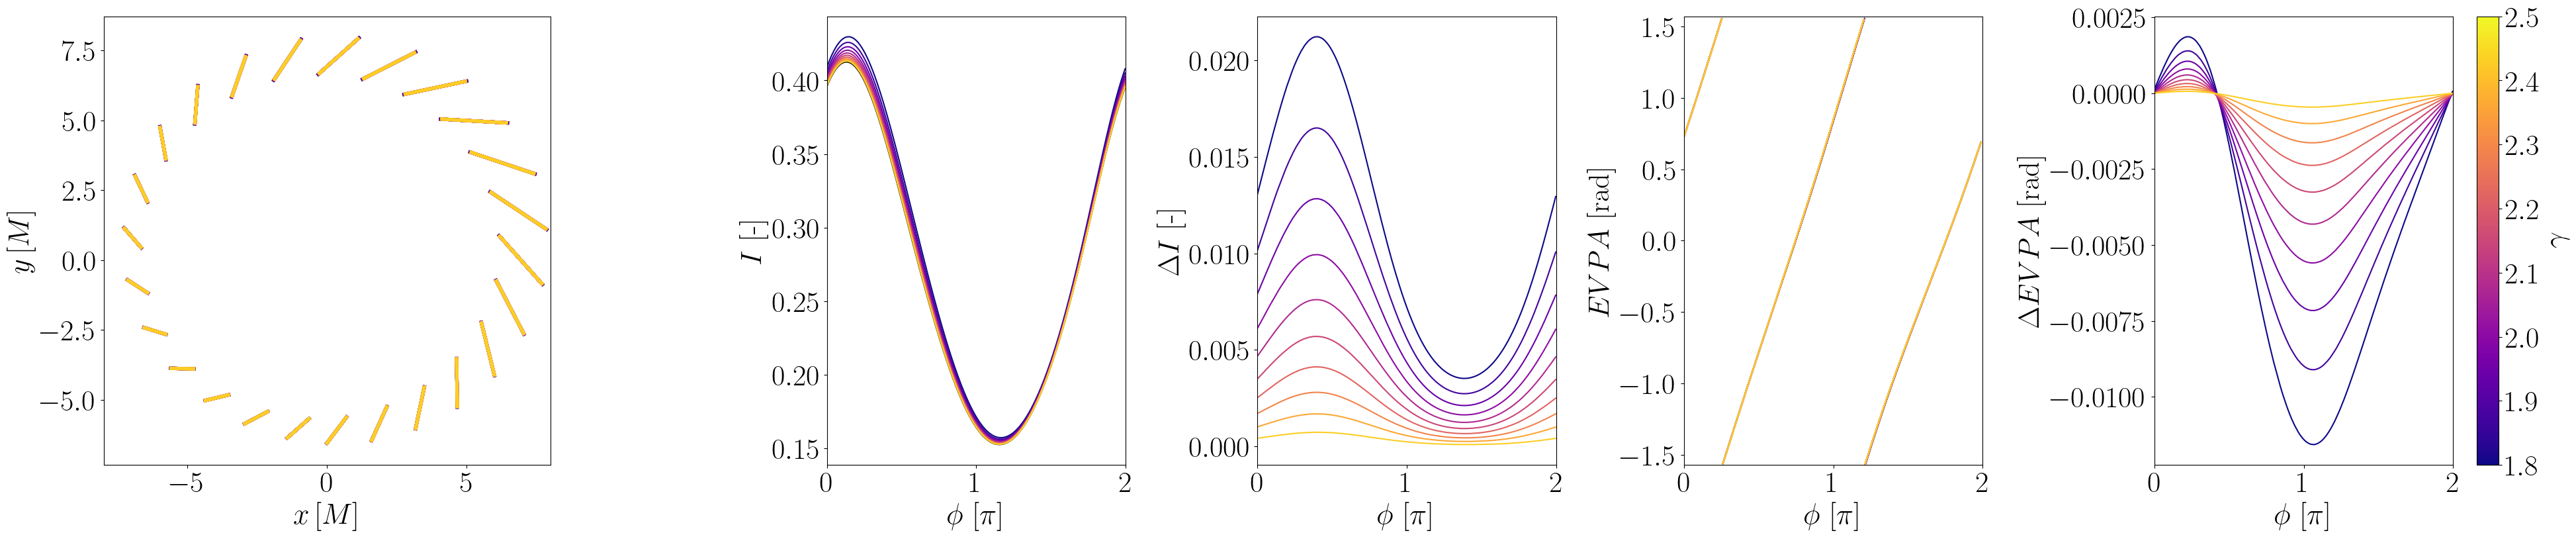
\includegraphics[scale = 0.13]{JNW_delta_figs_B_0.71_0.0_0.71_20_deg_direct.png}
		\caption{$\vec{B} = [0.71, 0, 0.71]$, $\beta = 0.3$, $\chi = -135^\circ$.}
	\end{subfigure}\\
	\begin{subfigure}{12cm}
		\hspace{-0.25cm}
		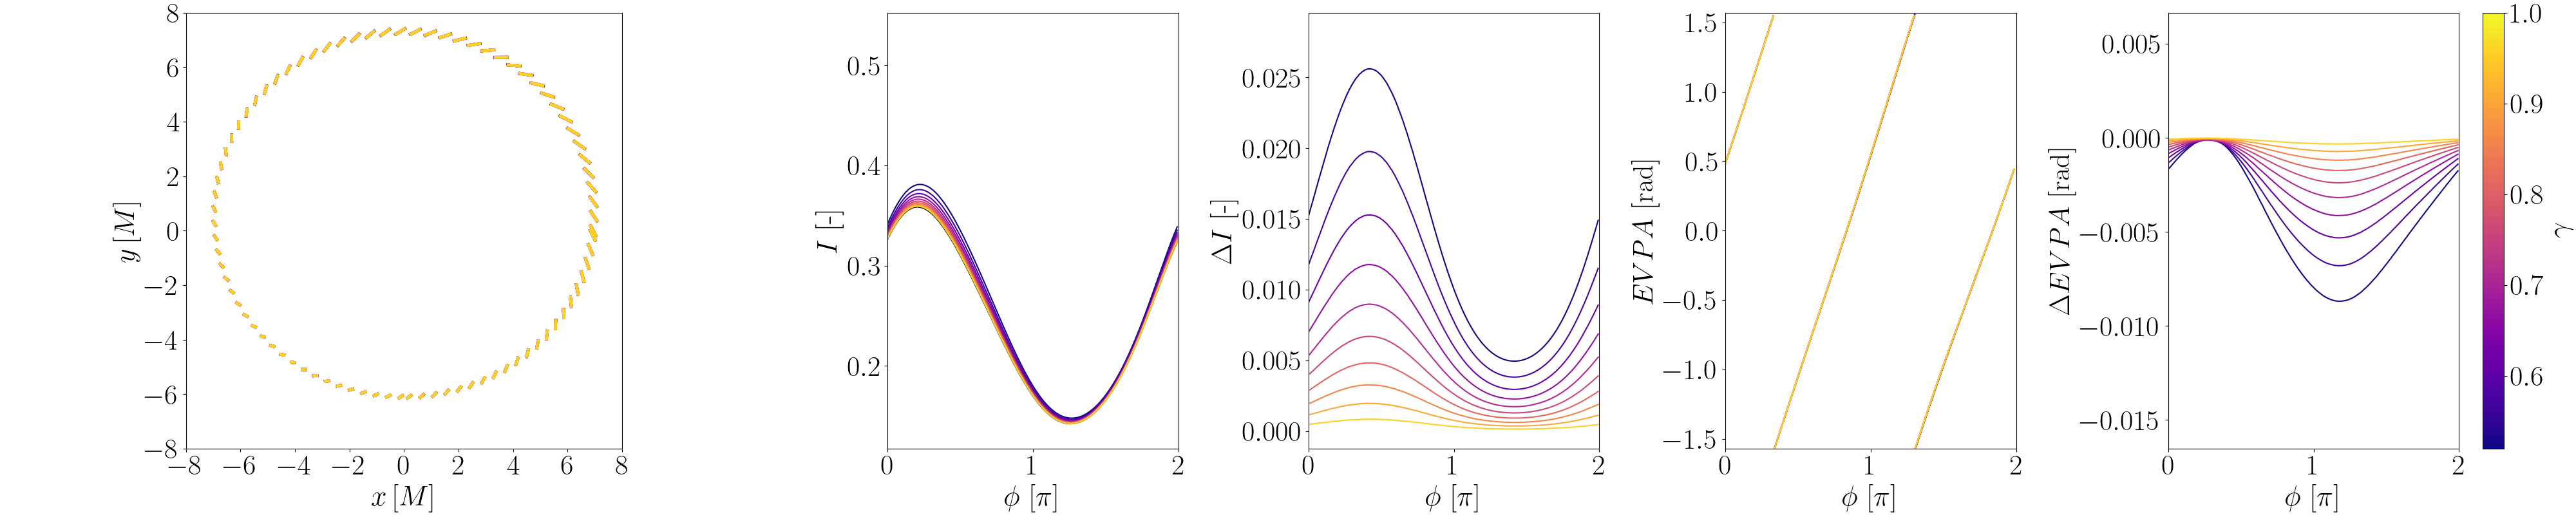
\includegraphics[scale = 0.13]{JNW_delta_figs_B_0.87_0.0_0.5_20_deg_direct.png}
		\caption{$\vec{B} = [0.87, 0, 0.5]$, $\beta = 0.3$, $\chi = -150^\circ$.}
	\end{subfigure}
	\caption[Профили на отклоненията на директните поляризирани образи oт тип $\{x,y\}\vert_{6M, \text{Schw}}$, за $i = 20\deg$ за голи сингуларности на Джанис-Нюман-Уиникър.]{\small Профили на отклоненията на директните поляризирани образи от тип $\{x,y\}\vert_{6M, \text{Schw}}$, за голи сингуларности на Джанис-Нюман-Уиникър при $i = 20\deg$. Стойността $\gamma = 1$ съответства на черни дупки на Шварцшилд.} 
	\label{JNW_delta_r6_20_deg}
\end{figure}

Виждаме, че амплитудата на отклоненията са на порядък по-малки от тези на фигура \ref{WH_delta_r6}. Виждаме, че $\Delta I$ расте при увеличаване на радиалната компонента на магнитното поле, докато отклонението на наклона на поляризационният вектор спада. Максималното относително отклонение по интензитет, което наблюдаваме е не-повече от $7.5\%$, докато по наклон е не-повече от $1.5\%$. За най-добрия кандидат магнитно поле, което описва наблюденията на М87$^*$ - $\vec{B} = [0.87, 0, 0.5]$, всички стойности на $\gamma$ дават практически еднакъв наклон на поляризационния вектор с черни дупки на Шварцшилд ($\max \Delta EVPA / EVPA_\text{Schw}<0.7\%$).\newpage

За пълнота изследваме и директните образи при високи инклинации ($i = 70^\circ$). Резултатите са представени на фигура \ref{JNW_delta_r6_70_deg}.

\begin{figure}[!htb]
	\centering
	\begin{subfigure}{12cm}
	\hspace{-0.25cm}
	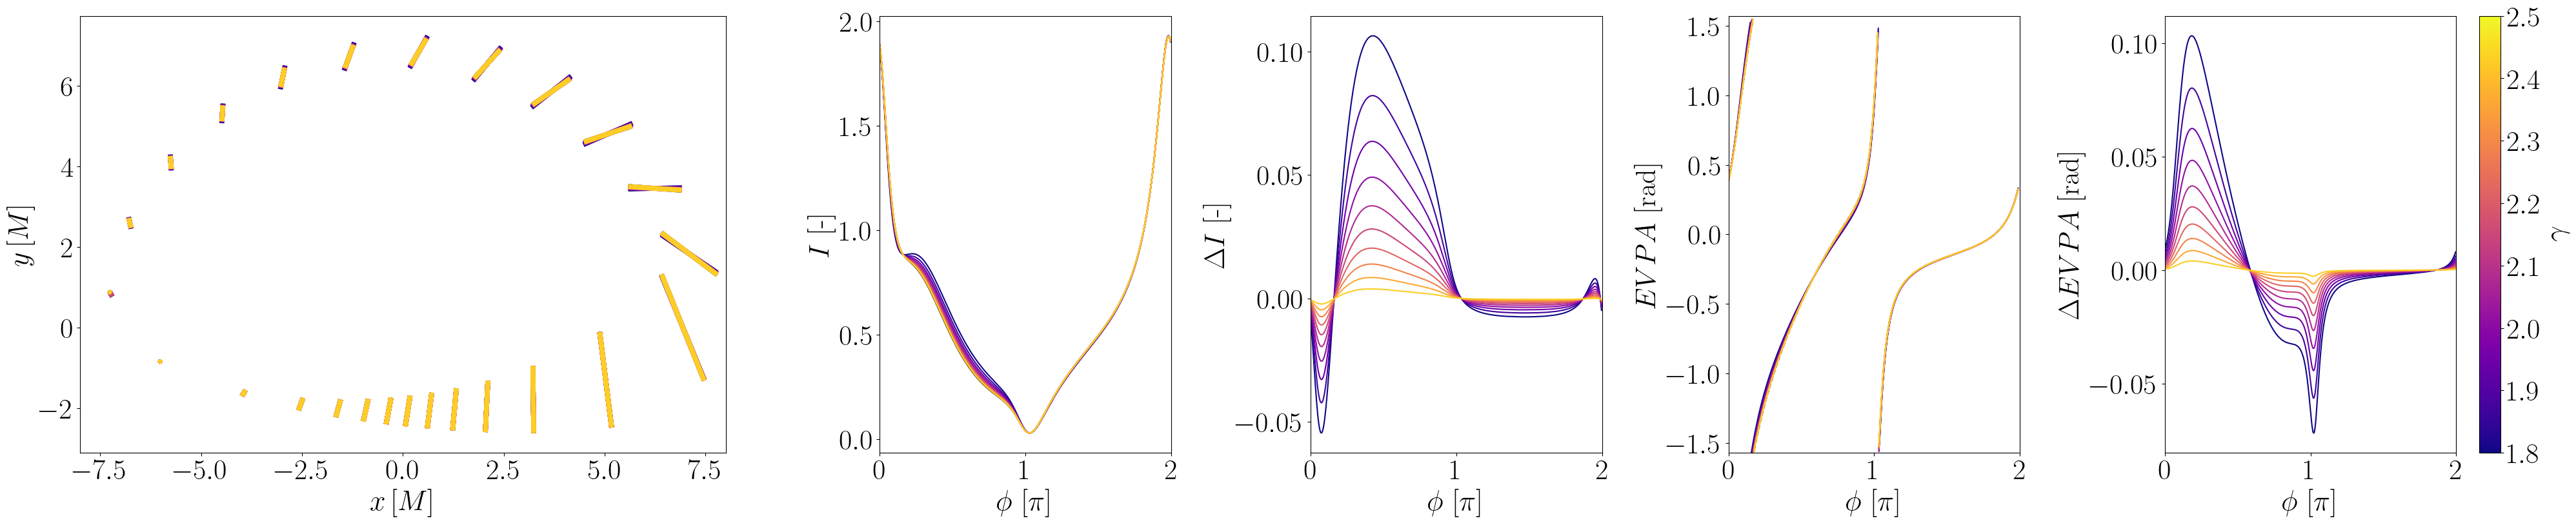
\includegraphics[scale = 0.13]{JNW_delta_figs_B_0.5_0.0_0.87_70_deg_direct.png}
	\caption{$\vec{B} = [0.5, 0, 0.87]$, $\beta = 0.3$, $\chi = -120^\circ$.}
\end{subfigure}\\
\begin{subfigure}{12cm}
	\hspace{-0.25cm}
	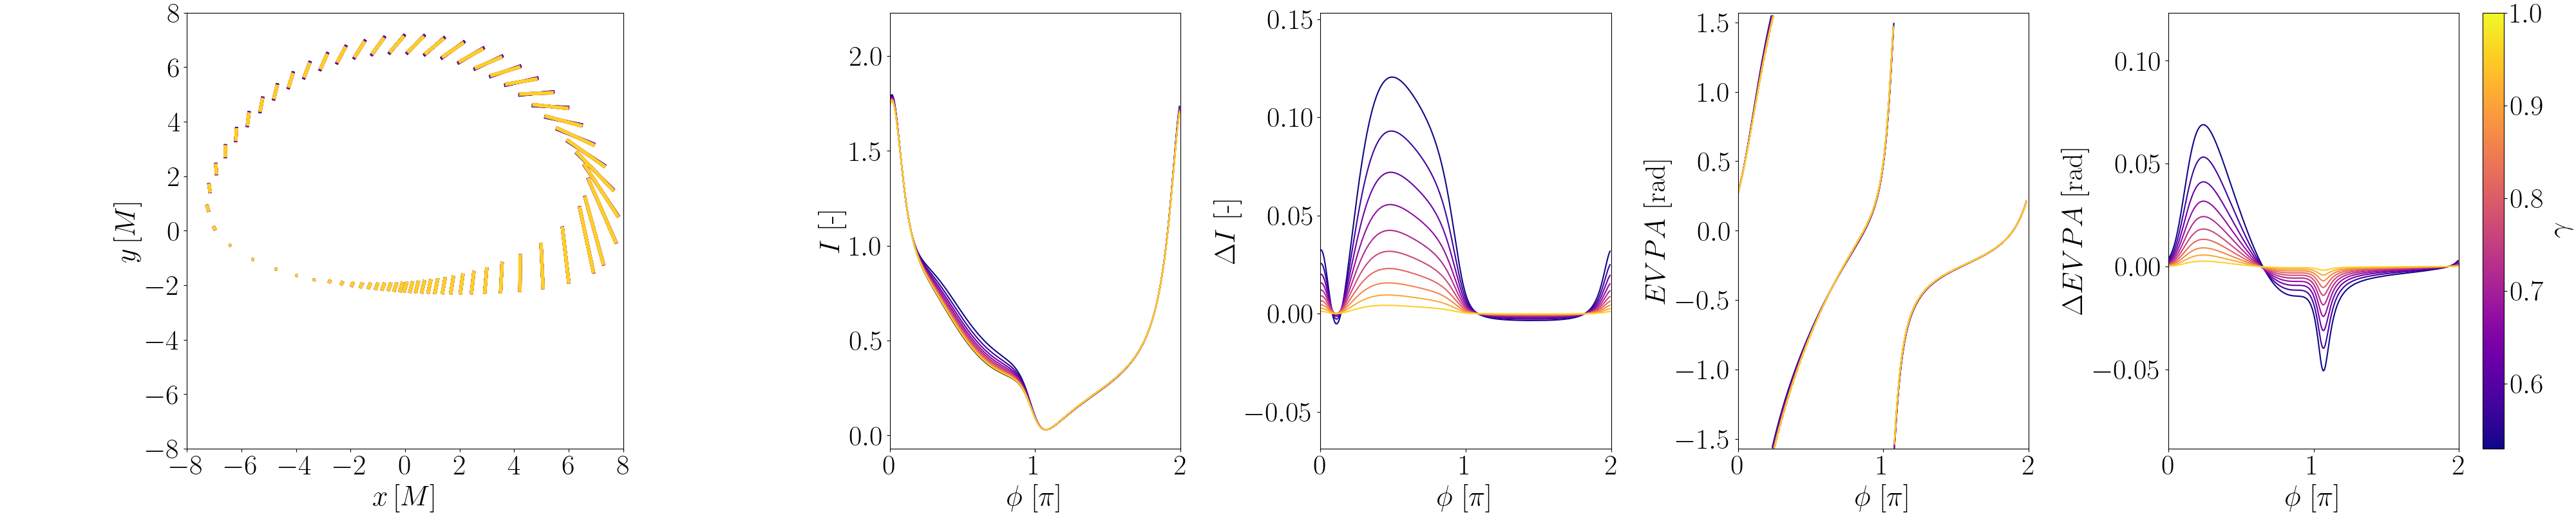
\includegraphics[scale = 0.13]{JNW_delta_figs_B_0.71_0.0_0.71_70_deg_direct.png}
	\caption{$\vec{B} = [0.71, 0, 0.71]$, $\beta = 0.3$, $\chi = -135^\circ$.}
\end{subfigure}\\
\begin{subfigure}{12cm}
	\hspace{-0.25cm}
	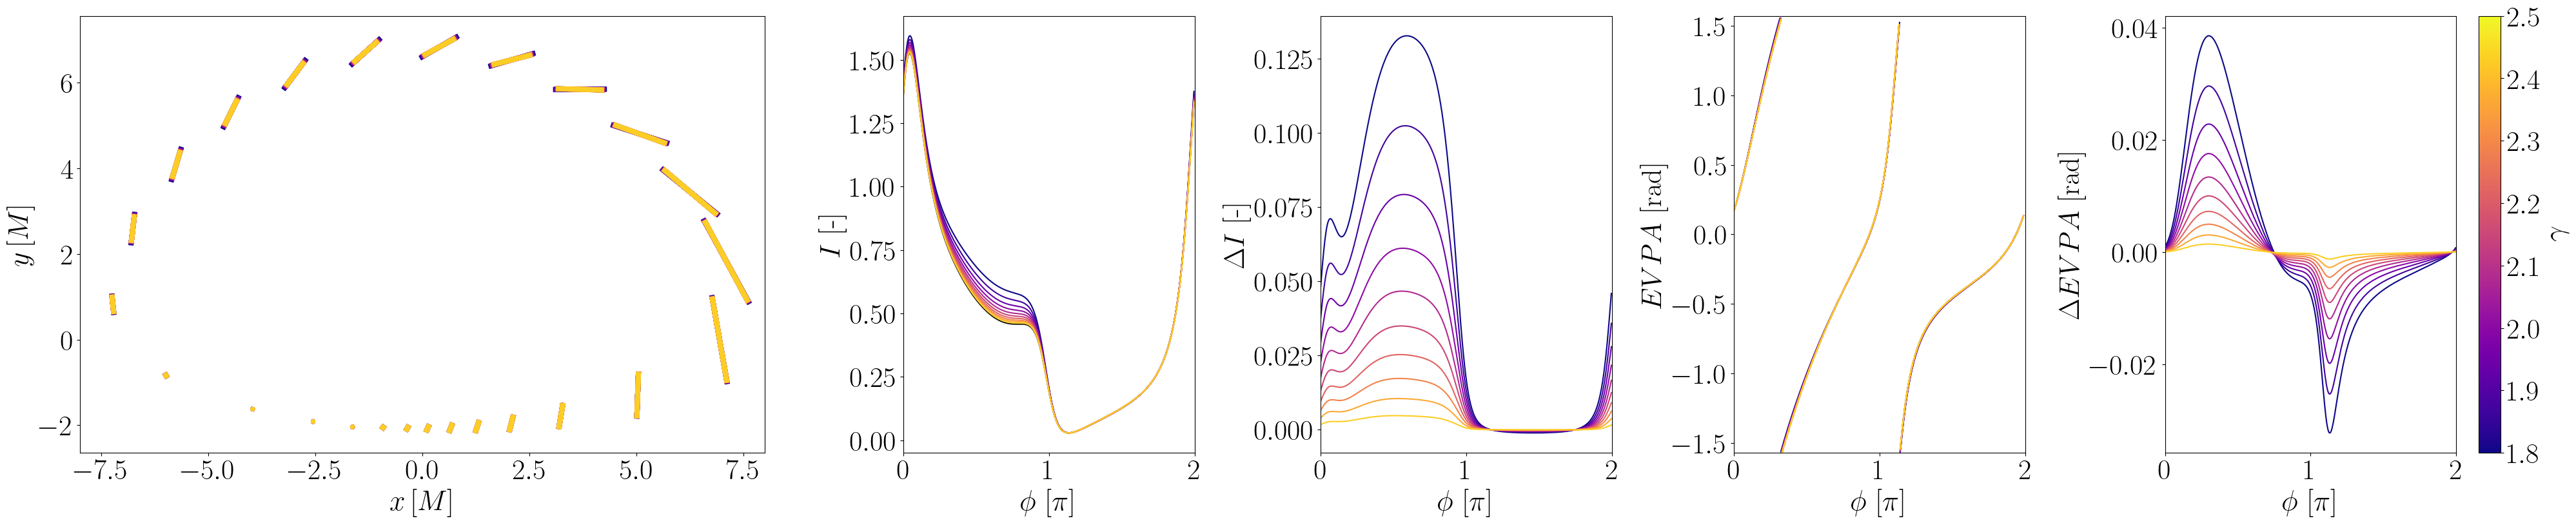
\includegraphics[scale = 0.13]{JNW_delta_figs_B_0.87_0.0_0.5_70_deg_direct.png}
	\caption{$\vec{B} = [0.87, 0, 0.5]$, $\beta = 0.3$, $\chi = -150^\circ$.}
\end{subfigure}
	\caption[Профили на отклоненията на директните поляризирани образи oт тип $\{x,y\}\vert_{6M, \text{Schw}}$, за $i = 70\deg$ за голи сингуларности на Джанис-Нюман-Уиникър.]{\small Профили на отклоненията на директните поляризирани образи от тип $\{x,y\}\vert_{6M, \text{Schw}}$, за голи сингуларности на Джанис-Нюман-Уиникър при $i = 70\deg$. Стойността $\gamma = 1$ съответства на черни дупки на Шварцшилд.} 
	\label{JNW_delta_r6_70_deg}
\end{figure}
Забелязваме, както при тунела, че отклоненията в този случай се увеличават. Максималното относително отклонение по интензитет достигаме за магнитно поле $\vec{B} = [0.87,0,0.5]$ - $26.5\%$, докато по наклон - $6.8\%$, при магнитно поле $0.5, 0.87, 0$. Резултатите за двете инклинации $i = \{20^\circ, 70^\circ\}$ са обобщени в таблици \ref{table:JNW_theta20} и \ref{table:JNW_theta70} за $\gamma = 0.53$, при която наблюдаваме най-големите отклонения от Шварцшилд.

\newpage

\begin{table}
	\centering
	\begin{tabular}{||c|c|c|c||}
		\hline
		\thead{ Магнитно поле }   &  \thead{$\left(\frac{\text{max}\,\Delta \text{I}}{\text{I}_\text{Sch}} \, [\%], \, \phi \, [rad]\right)$} & \thead{$\left(\frac{\text{max}\,\Delta \text{EVPA}}{\text{EVPA}_\text{Sch}} \, [\%] , \, \phi \, [rad]\right)$} & $\gamma$
		\\  \hline
		
		\thead{\vspace{0.1mm}$\vec{B}\text{ = [0.5, 0.87, 0]}$\vspace{0.1mm}  }   &  \thead{(4.385, 0.385$\pi$)} & \thead{(1.221, 0.986$\pi$)} & \thead{0.530}
		\\  \hline
		
		\thead{\vspace{0.1mm}$\vec{B}\text{ = [0.71, 0.71, 0]}$\vspace{0.1mm}} &  \thead{(5.928, 0.397$\pi$)} & \thead{(1.076, 1.066$\pi$)} & \thead{0.530}
		\\  \hline
		
		\thead{\vspace{0.1mm}$\vec{B}\text{ = [0.87, 0.5, 0]}$\vspace{0.1mm}} &  \thead{(7.331, 0.421$\pi$)} & \thead{(0.716, 1.178$\pi$)} & \thead{0.530}
		\\  \hline          
	\end{tabular}
	\caption[Максималните относителни отклонения на директните поляризирани образи на голи сингулярности на Джанис-Нюман-Уиникър при $i = 20^\circ$ и $\gamma = 0.53$]{Максималните относителни на директните поляризирани образи на голи сингулярности на Джанис-Нюман-Уиникър при $i = 20^\circ$ и $\gamma = 0.53$}
	\label{table:JNW_theta20}
\end{table}

\begin{table}[]
	\centering
	\begin{tabular}{||c|c|c|c||}
		\hline
		\thead{ Магнитно поле }   &\thead{$\left(\frac{\text{max}\,\Delta \text{I}}{\text{I}_\text{Sch}} \, [\%], \, \phi \, [rad]\right)$} & \thead{$\left(\frac{\text{max}\,\Delta \text{EVPA}}{\text{EVPA}_\text{Sch}} \, [\%] , \, \phi \, [rad]\right)$} & $\gamma$
		\\  \hline
		
		\thead{\vspace{0.1mm}$\vec{B}\text{ = [0.5, 0.87, 0]}$\vspace{0.1mm}}  &  \thead{(18.00, 0.429$\pi$)} & \thead{(6.809, 0.184$\pi$)} & \thead{0.530}
		\\  \hline
		
		\thead{\vspace{0.1mm}$\vec{B}\text{ = [0.71, 0.71, 0]}$\vspace{0.1mm}} &  \thead{(22.65, 0.497$\pi$)} & \thead{(4.482, 0.240$\pi$)} & \thead{0.530}
		\\  \hline
		
		\thead{\vspace{0.1mm}$\vec{B}\text{ = [0.87, 0.5, 0]}$\vspace{0.1mm}}  &  \thead{(26.45, 0.593$\pi$)} & \thead{(2.629, 0.301$\pi$)} & \thead{0.530}
		\\  \hline
	\end{tabular}
	\caption[Максималните относителни на директните поляризирани образи на голи сингулярности на Джанис-Нюман-Уиникър при $i = 70^\circ$ и $\gamma = 0.53$]{Максималните относителни на директните поляризирани образи на голи сингулярности на Джанис-Нюман-Уиникър при $i = 70^\circ$ и $\gamma = 0.53$}
	\label{table:JNW_theta70}
\end{table}

\subsubsection{Поляризация на индиректните образи}

\begin{minipage}{16em}
	\hspace{-0.3cm}
	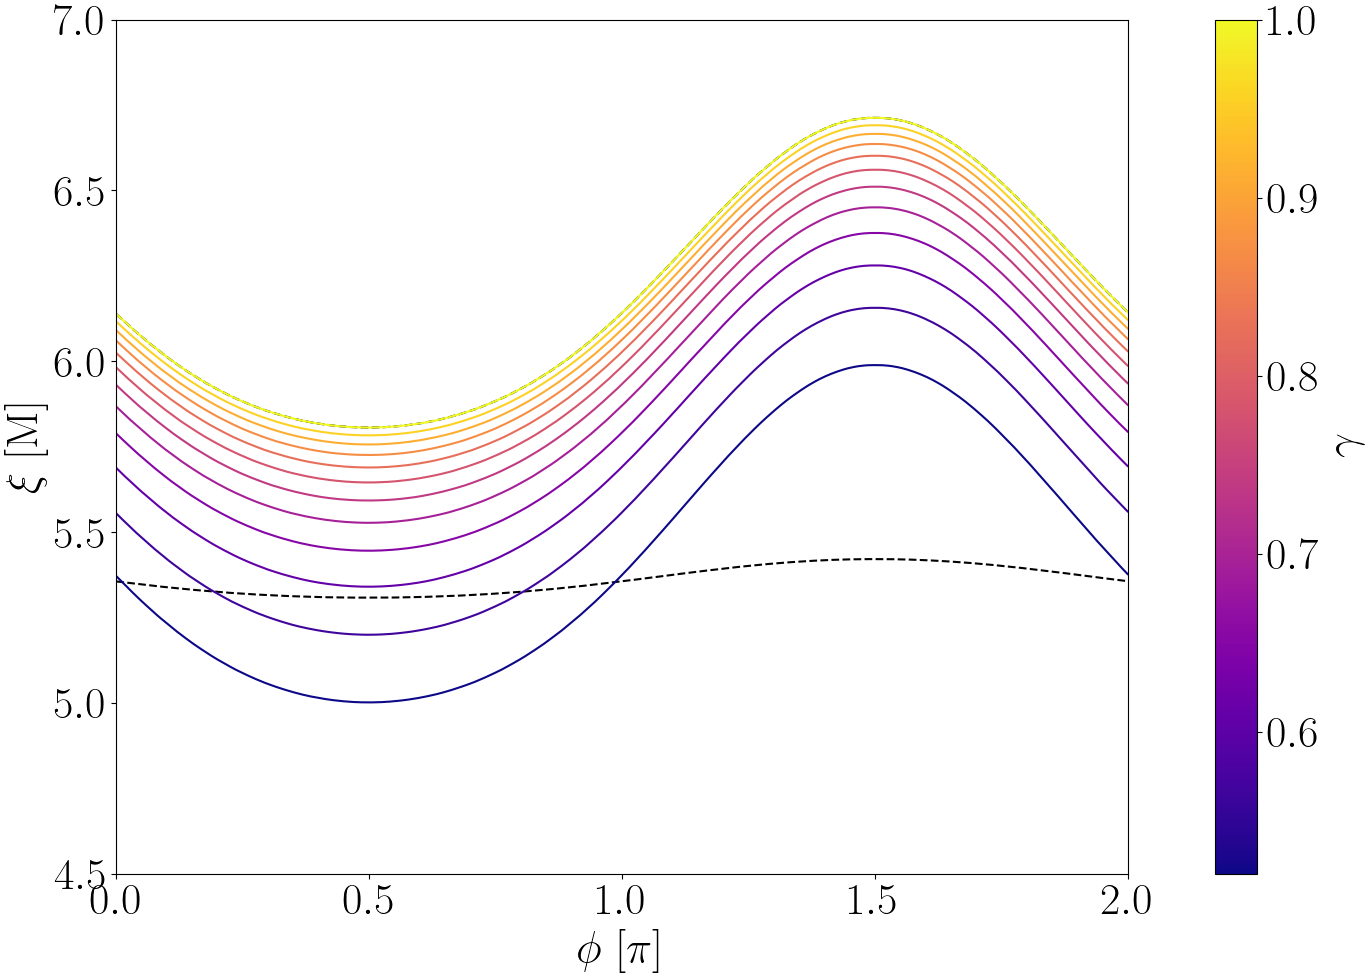
\includegraphics[scale = 0.18]{JNW_indirect_overlap_grapth.png}
	\captionof{figure}[Диаграма на формиране на образи от тип $\{x,y\}\vert_{X, \text{Schw}}$ за голи сингулярности на Джанис-Нюман-Уиникър]{Диаграма на формиране на образи от тип $\{x,y\}\vert_{X, \text{Schw}}$ за голи сингулярности на Джанис-Нюман-Уиникър. Виждаме, че приблизителният диапазон на съществуване е $0.6 \lessapprox \gamma \le 1$.} 
	\label{JNW_n1_overlap}
\end{minipage}\,\,
\begin{minipage}{20em}
	Нека сега разгледаме и образите от тип $\{x,y\}\vert_{X, \text{Schw}}$ с $n = 1$. Както случая при тунела, тe съществуват само за определен интервал на метричният параметър $\gamma$. Фигура \ref{JNW_n1_overlap} изобразява графично условието им за съществуване (7.28а), понеже (7.28б) е изпълнено само за $\gamma = 1$. Можем да видим, че при  $0.6 \lessapprox \gamma \le 1$, (7.28a) е изпълнено. Анализът ни на отклоненията от Шварцшилд за този интервал на $\gamma$ e показан на фигура \ref{JNW_delta_r6_20_deg_n1} за $X = 6M$ и $\gamma\in(0.62, 1]$ (което е интервалът, в който численият код Mjølnir намира образи).
\end{minipage}\\

Причината да изключим стойността $\gamma = 0.62$ от фигура \ref{JNW_delta_r6_20_deg_n1} e, че при стойности на $\gamma$, клонящи към граничната, за формиране на образи от тип $\{x,y\}\vert_{X, \text{Schw}}$, относителното отклонение в интензитета расте изключително бързо. Минималната стойност на $\gamma$ във фигура \ref{JNW_delta_r6_20_deg_n1} е $\gamma = 0.623838$, при която за магнитно поле $\vec{B} = [0.5, 0, 0.87]$ относителното отклонение в интензитета достига $\approx 600\%$. За $\gamma = 0.62$ обаче, имаме относително отклонение в интензитета $\approx 6\times 10^3 \%$.\\

При формирането на тези образи за ниски стойности на $\gamma$ обаче, фотоните попадат върху диска при много високи радиални координати $r_s\approx 10^3M$, където не се очаква да има значителен принос на излъчването. Възможно е това да компенсира ефекта на пространство-времето и по-реалистичен модел на излъчващата среда да \emph{не} предсказва подобни нараствания в интензитета. \\

Абстрахирайки се от тези гранични стойности на $\gamma$, можем да заключим, че както при тунела, амплитудата на отклоненията от Шварцшилд нараства значително за тези образи. 

\begin{figure}[!htb]
	\centering
	\begin{subfigure}{12cm}
		\hspace{-0.25cm}
		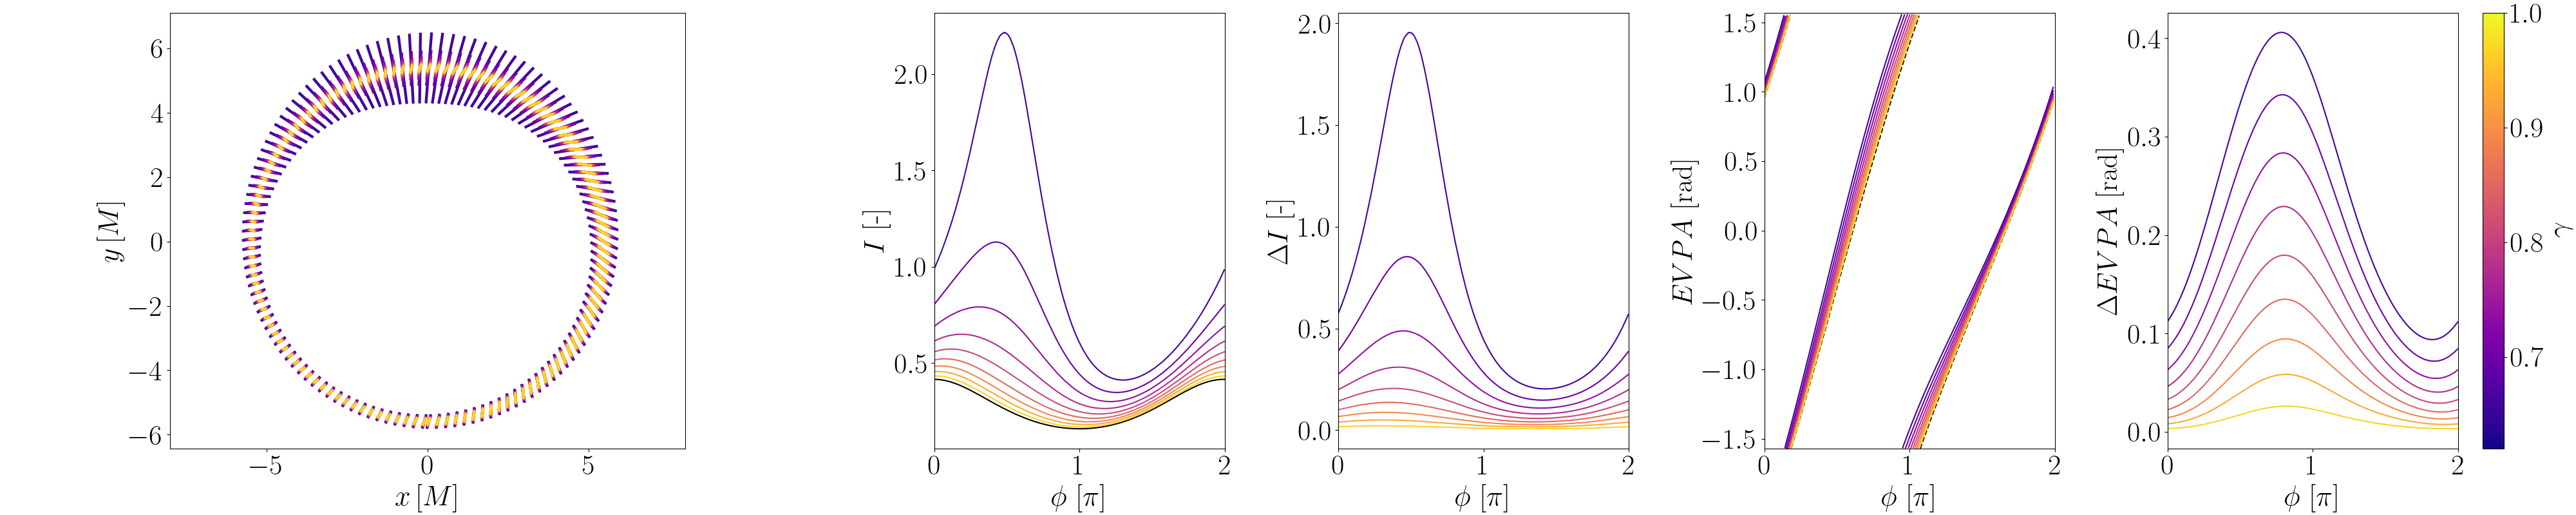
\includegraphics[scale = 0.13]{JNW_delta_fig_B_0.5_0.87_0_20_deg_r6_n1.png}
		\caption{$\vec{B} = [0.5, 0, 0.87]$, $\beta = 0.3$, $\chi = -120^\circ$.}
	\end{subfigure}\\
	\begin{subfigure}{12cm}
		\hspace{-0.25cm}
		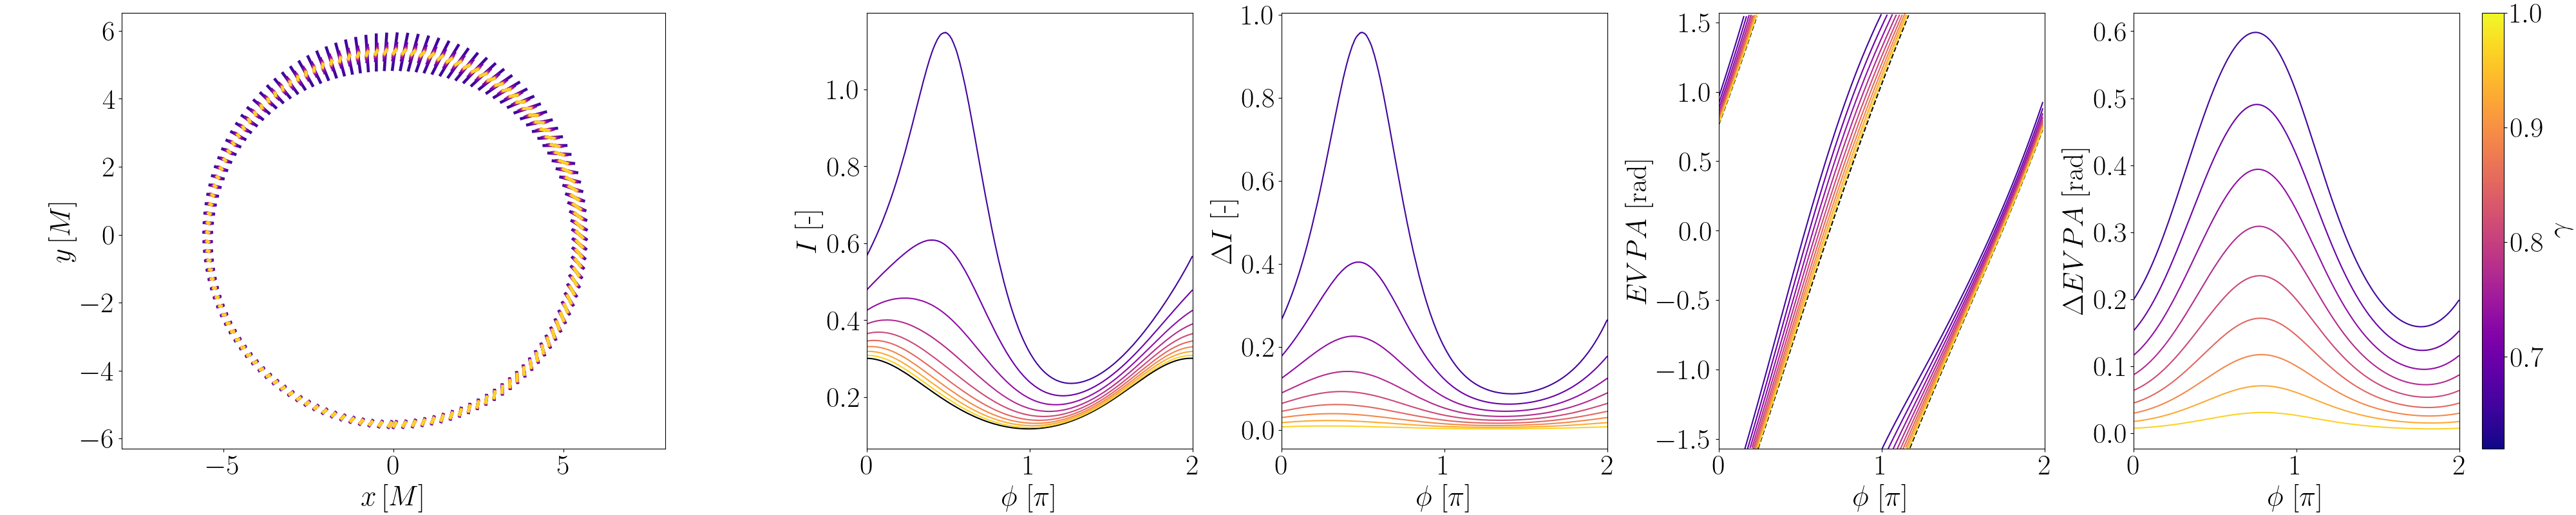
\includegraphics[scale = 0.13]{JNW_delta_fig_B_0.71_0.71_0_20_deg_r6_n1.png}
		\caption{$\vec{B} = [0.71, 0, 0.71]$, $\beta = 0.3$, $\chi = -135^\circ$.}
	\end{subfigure}\\
	\begin{subfigure}{12cm}
		\hspace{-0.25cm}
		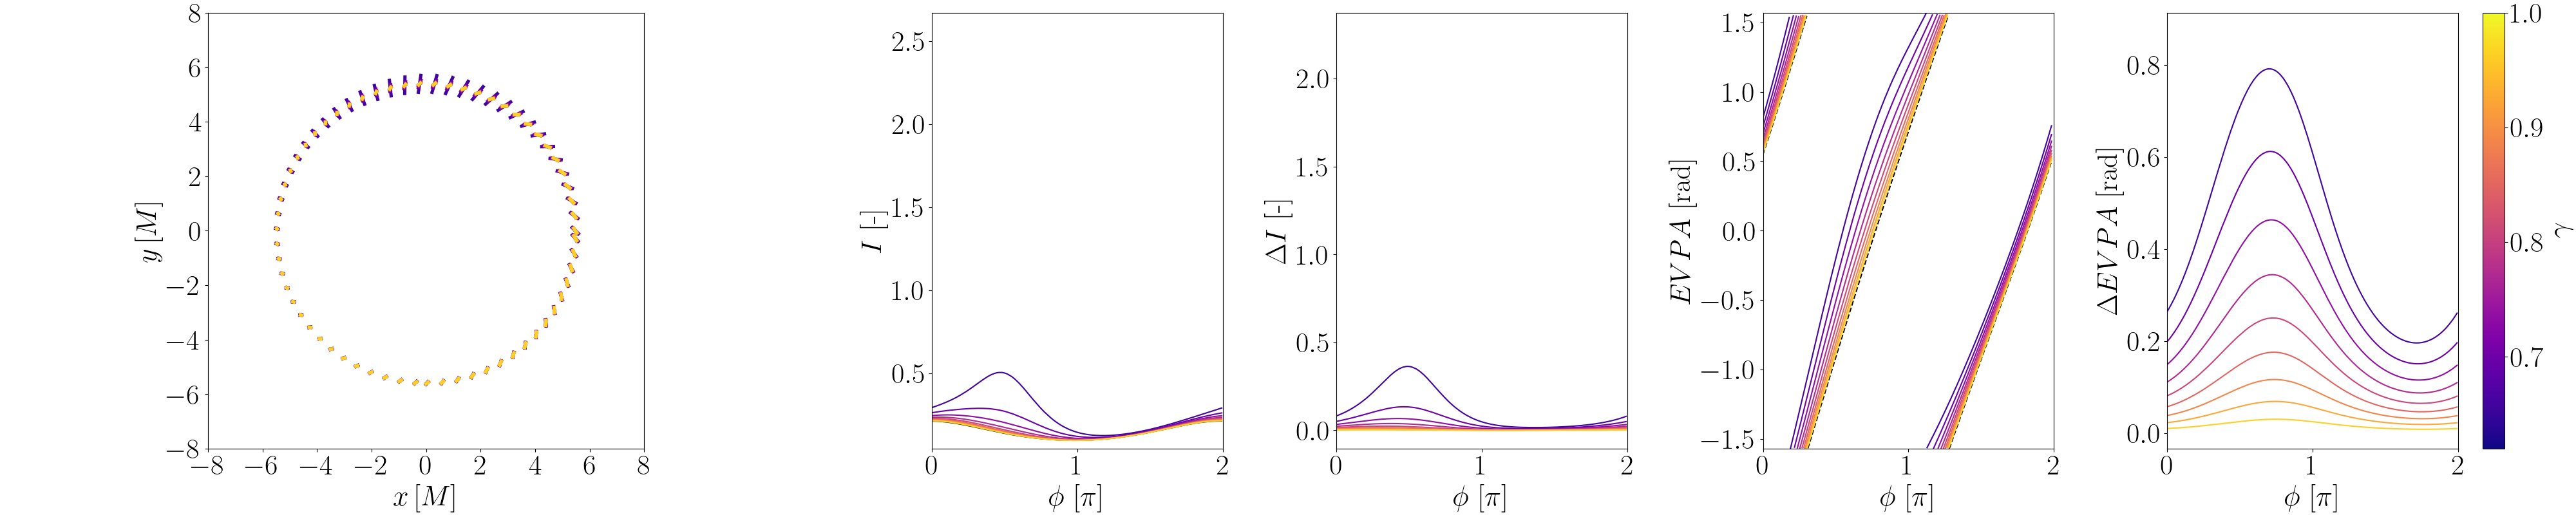
\includegraphics[scale = 0.13]{JNW_delta_fig_B_0.87_0.5_0_20_deg_r6_n1.png}
		\caption{$\vec{B} = [0.87, 0, 0.5]$, $\beta = 0.3$, $\chi = -150^\circ$.}
	\end{subfigure}
	\caption[Профили на отклоненията на $n = 1$ поляризирани образи oт тип $\{x,y\}\vert_{6M, \text{Schw}}$, за $i = 20\deg$ за голи сингуларности на Джанис-Нюман-Уиникър.]{\small Профили на отклоненията на $n = 1$ поляризирани образи от тип $\{x,y\}\vert_{6M, \text{Schw}}$, за голи сингуларности на Джанис-Нюман-Уиникър при $i = 70\deg$. Стойността $\gamma = 1$ съответства на черни дупки на Шварцшилд.} 
	\label{JNW_delta_r6_20_deg_n1}
\end{figure}

Виждаме, както при тунела, че при тези образи се проявява и качествена морфологична разлика спрямо Шварцшилд. Видимата позиция на максимума на интензитета се измества към горната част на образа $\phi = \pi / 2$, с намаляване на скаларният параметър $\gamma$.